\documentclass[
  reprint,
  superscriptaddress,
  amsmath,
  amssymb,
  aps,
  pre,
  nofootinbib,
  floatfix
]{revtex4-2}

\usepackage[T1]{fontenc}
\usepackage[cal=boondoxo]{mathalpha}
\usepackage{graphicx}
\usepackage{microtype}
\setlength{\emergencystretch}{2em}
\widowpenalty=600
\clubpenalty=600
% Long multi-line displays are the only unbreakable blocks in the appendices;
% letting them split when a column runs out avoids large holes above them.
\allowdisplaybreaks[1]

\newcommand{\rv}{\vec r}
\newcommand{\ev}{\hat{n}}
\newcommand{\evp}{\hat{n}_{\perp}}
\newcommand{\pv}{\vec p}
\newcommand{\nv}{\hat\nu}
\newcommand{\Wv}{\vec W}
\newcommand{\Jrho}{\vec J_{\rho}}
\newcommand{\uv}{\mathbf u}
\newcommand{\Rv}{\mathbf R}
\newcommand{\Qt}{\mathbf Q}
\newcommand{\Id}{\mathbf I}
\newcommand{\grad}{\vec{\nabla}}
\newcommand{\lap}{\nabla^2}
\newcommand{\dd}{\mathrm d}
\newcommand{\ord}{\mathcal O}
\newcommand{\Ud}{\mathbb D}
\newcommand{\pnormal}{\partial_{\nu}}
\newcommand{\Pturn}{\mathcal P_{\mathrm{turn}}}
\newcommand{\Pturntwo}{\mathcal P_{2,\mathrm{turn}}}
\newcommand{\DR}{\mathcal D_R^{(0)}}
\newcommand{\DRtwo}{\mathcal D_{R,2}^{(0)}}
\newcommand{\zp}{\zeta_\parallel}
\newcommand{\Pnet}{\vec P}
\newcommand{\Xc}{\vec X}
\newcommand{\Erho}{\mathcal E_\rho}
\newcommand{\Crho}{\mathcal C_\rho}
\newcommand{\Gp}{\mathcal G_p}
\newcommand{\Cp}{\mathcal C_p}
\newcommand{\Irate}{\mathcal I}
\newcommand{\Gv}{\vec{\mathcal G}_\rho}
\newcommand{\Piv}{\vec{\mathcal E}_p}
\newcommand{\Tsh}{\mathbf T}
\DeclareMathOperator{\Var}{Var}

% Each results section ends with a compact readout: what to look for in the
% data, and what seeing it implies.  These sit in the text flow rather than
% floating, so a reader can find the recipe beside the physics that justifies
% it.
\newenvironment{readout}
  {\par\addvspace{1.2ex}\noindent\rule{\columnwidth}{0.6pt}\par\nobreak
   \vspace{0.3ex}\noindent\textbf{Reading it off the data}\par\nobreak
   \vspace{0.4ex}\footnotesize\noindent
   \setlength{\parindent}{0pt}\emergencystretch=2em\relax
   \begin{tabular}{@{}p{0.40\columnwidth}@{\hspace{1em}}p{0.49\columnwidth}@{}}}
  {\end{tabular}\par\nobreak\vspace{0.4ex}%
   \noindent\rule{\columnwidth}{0.6pt}\par\addvspace{1.0ex}}

% The bibliography is written explicitly below.  Disable REVTeX's automatic
% endnote bibliography and its Notes.bib output stream so that external BibTeX
% is not invoked during compilation (including under TeX Live 2025).
\makeatletter
\let\auto@bib\@empty
\let\auto@bib@innerbib\@empty
\let\write@bibliographystyle\relax
\let\@bibdataout@init\relax
\makeatother

% Float placement.  Five full-width figures fall inside one short section, and
% a double-column float can only reach the top of a page, so the defaults queue
% them well past the text that cites them.  These let two share a page top.
% The raised \floatpagefraction also stops a tall single-column figure from
% claiming a whole column to itself and leaving the text below it blank.
\setcounter{topnumber}{3}
\setcounter{dbltopnumber}{3}
\setcounter{totalnumber}{4}
\renewcommand{\topfraction}{0.92}
\renewcommand{\dbltopfraction}{0.92}
\renewcommand{\bottomfraction}{0.5}
\renewcommand{\textfraction}{0.06}
\renewcommand{\floatpagefraction}{0.90}
\renewcommand{\dblfloatpagefraction}{0.85}

% Vertical rhythm.  The class defaults leave a wide band of white around
% floats and headings; these bring the page back to a compact, even texture.
\setlength{\textfloatsep}{12pt plus 3pt minus 3pt}
\setlength{\dbltextfloatsep}{12pt plus 3pt minus 3pt}
\setlength{\floatsep}{10pt plus 2pt minus 2pt}
\setlength{\dblfloatsep}{10pt plus 2pt minus 2pt}
\setlength{\intextsep}{10pt plus 2pt minus 2pt}
\setlength{\abovecaptionskip}{5pt}

\makeatletter
\def\section{\@startsection{section}{1}{\z@}%
  {0.50cm \@plus1ex \@minus.3ex}{0.28cm}%
  {\normalfont\small\bfseries\hyphenpenalty=10000\exhyphenpenalty=10000}}%
\def\subsection{\@startsection{subsection}{2}{\z@}%
  {0.45cm \@plus1ex \@minus.3ex}{0.25cm}%
  {\normalfont\small\bfseries\hyphenpenalty=10000\exhyphenpenalty=10000}}%
\def\subsubsection{\@startsection{subsubsection}{3}{\z@}%
  {0.45cm \@plus1ex \@minus.3ex}{0.25cm}{\normalfont\small\itshape}}%
\makeatother

\begin{document}

\title{Which foraging strategy?  Reading microscopic motility rules from a
population release}

\author{Jairo M. Rojas}
\affiliation{Department of Physics, University of Illinois Urbana--Champaign,
Urbana, Illinois 61801, USA}
\affiliation{Department of Mechanical Science and Engineering, The Grainger
College of Engineering, University of Illinois Urbana--Champaign, Urbana,
Illinois 61801, USA}

\author{Naama Brenner}
\affiliation{The Wolfson Department of Chemical Engineering,
Technion--Israel Institute of Technology, Haifa 3200003, Israel}

\author{Ahmed El Hady}
\affiliation{Centre for the Advanced Study of Collective Behaviour,
University of Konstanz, 78464 Konstanz, Germany}
\affiliation{Department of Collective Behavior, Max Planck Institute of Animal
Behavior, 78464 Konstanz, Germany}

\date{\today}

\begin{abstract}
A population of cells that piles up where the food is does not thereby reveal
how it got there: many different microscopic responses to a nutrient produce
the same accumulation.  We ask which of them a release experiment---drop a
blob of cells and film it---can actually tell apart.  Nine elementary
responses, from tumbling less while headed up-gradient to simply swimming
slower in rich patches, fit inside one model of position and heading, which we
coarse-grain to equations for cell density and mean heading.  Four numbers a
film readily yields---where the cloud goes, how wide it gets, how elongated,
and which way it points---obey closed equations, and each response enters them
at its own power of time.  This sorts the nine into six distinguishable groups
and sets how long each must be watched.  Read once the cloud has stopped
moving, the same numbers separate two coefficients that are routinely
conflated: the cloud's width returns the chemotactic mobility, its elongation
returns the drift of its centre of mass, and the two can differ in sign.  It
is the mobility, not the drift, that fixes how much nutrient the population
eats and how densely it accumulates---and it does so on the food's diffusive
time rather than the dish's, so foraging finishes long before the density
settles.  Tracking single cells over a fixed lag supplies the remaining
combinations and separates navigating well from moving informatively: the two
responses that never carry a cell up-gradient are the two its motion reveals
the most about.  We tabulate what each measurement returns, and verify every
prediction against particle simulations and a conservative finite-volume
solution with no fitted transport coefficient.
\end{abstract}

\maketitle

\section{Introduction}
\label{sec:introduction}

Suppose you find a dish of bacteria heaped up on a patch of food.  What have
you learned?  Less than you might think.

A cell has more than one knob to turn.  More nutrient may make it swim faster,
jiggle more, hold its heading longer, tumble less often, or bias the turns it
does make---and any one of these can end with the population sitting where the
food is.  Some of them involve no sense of direction whatever: a cell that
merely slows down in a rich patch will accumulate there, for the same reason
that traffic piles up where the road is slow.  The heap is real, but it is not
by itself evidence of chemotaxis.

The converse is just as awkward.  A response that plainly changes how
individual cells move can leave the population's centre of mass exactly where
it started.

Two questions follow.  \emph{Forward}: how does each way of modulating
motility change what the population does?  \emph{Inverse}---the one an
experimenter actually faces---which of them can be told apart, from what
measurement, and after how long?  Run-and-tumble motion and its continuum
limits supply a natural language for
both~\cite{berg1972,schnitzer1993,tailleur2008}; related work has asked how
information constraints shape discrete navigation
strategies~\cite{betancourt2026}.

We answer both by fixing the nutrient landscape and following each response
through to the population it produces.  Nine elementary rules turn out to live
inside a single model of position and heading (Sec.~\ref{sec:overview}),
which we coarse-grain to equations for the two
fields an imaging experiment can reconstruct---the cell density and the mean
heading (Sec.~\ref{sec:closure}).  Integrating those equations over space
closes a small system for the handful of numbers a release experiment actually
reports (Sec.~\ref{sec:observables}).

Everything after that is a question of \emph{when you look}.  Early, while the
cloud is still growing, each rule enters at its own power of time, and those
exponents sort the nine into six distinguishable groups and fix how long each
must be filmed (Sec.~\ref{sec:observable-hierarchy}).  Late, once the cloud
has stopped moving, the nine collapse onto a few transport numbers---among
them two that are routinely conflated: a mobility that says where the cells
end up and how much they eat, and a drift that says where their centre of mass
went.  The settled cloud's width returns the first and its elongation the
second, and for a speed rule the two have opposite signs
(Secs.~\ref{sec:long-time}--\ref{sec:foraging}).  Finally, tracking single
cells over a fixed lag supplies the combinations the fields merge, and
separates navigating well from moving informatively
(Sec.~\ref{sec:information}).  Section~\ref{sec:model-comparison} tests every
prediction against particle simulations and a finite-volume solution of the
coarse-grained equations.

The outcome is a field guide (Table~\ref{tab:inversion}, in
Appendix~\ref{app:observables}): each row a measurement you can make, and the
mechanisms it distinguishes.  A reader who wants the recipe rather than the
derivation can start there and work backwards; Table~\ref{tab:cases} names
the nine rules.  Appendices~\ref{app:model}--\ref{app:remaining-cases} carry
the derivations, the propagator and the numerics.

\section{Nine ways to respond}
\label{sec:overview}

Our setting is deliberately spare: $N$ noninteracting cells of one species in
a planar disk of radius $\mathcal R$, swimming through a smooth, static,
dimensionless nutrient field $\eta$ (Fig.~\ref{fig:case1-validation}).  The landscape shapes how the cells move;
the cells neither deplete nor replenish it.  Lengths are measured in
$\mathcal R$ and times in $\mathcal R^{2}/\mathcal D_T^{(0)}$, so that
$D_T^{(0)}=1$ and $\rv$ lives in the unit disk $\Ud$
(Appendix~\ref{app:model}).

A cell is a point $\rv\in\Ud$ with a heading $\ev(\theta)$, and it can read
three things about its surroundings.  The first is the \emph{local level}
$\delta\eta$, the nutrient excess over a uniform reference,
\begin{equation}
  \delta\eta(\rv)=\eta(\rv)-\eta^{(0)},
  \label{eq:deta}
\end{equation}

The other two are the components of the gradient resolved in the cell's own
body frame: the \emph{alignment signal} $\zp$ and the \emph{steering signal} $\zeta_\perp$,
\begin{equation}
  \zp(\rv,\theta)=\ev(\theta)\cdot\grad\eta(\rv),
  \qquad
  \zeta_\perp(\rv,\theta)=\evp(\theta)\cdot\grad\eta(\rv).
  \label{eq:signals}
\end{equation}

These three differ in what they can tell a cell.  Turning in place leaves
$\delta\eta$ unchanged, so a cell reading only the level knows how good its
present spot is but nothing about which way to go.  The alignment signal $\zp$
is positive when the cell is already headed toward food and negative when it
is headed away, so it grades the current heading.  The steering signal
$\zeta_\perp$ says which way to turn to improve.

Four coefficients set the motion: the \emph{speed} $v$, the
\emph{translational diffusivity} $D_T$ (how much the path jiggles), the
\emph{rotational diffusivity} $D_R$ (how fast the heading wanders), and the
\emph{tumbling rate} $\lambda$ (how often the cell reorients abruptly).  To
first order about their reference values,
\begin{equation}
\begin{split}
  X(\rv,\theta)&=X^{(0)}+X^{(\eta)}\delta\eta(\rv)
  +X^{(\zp)}\zp(\rv,\theta),\\
  &\hspace{20mm}X\in\{v,D_T,D_R,\lambda\},
\end{split}
  \label{eq:response}
\end{equation}
where the parenthesized superscripts label \emph{sensitivities}---how
strongly one signal tunes one coefficient---not powers.  Four coefficients
times two signals gives eight responses.  The steering signal cannot enter
this way: it changes sign under a reflection that a scalar coefficient cannot
see.  It therefore acts through a ninth mechanism, \emph{continuous steering} with signed sensitivity $\chi$,
\begin{equation}
  u_\theta(\rv,\theta)=\chi\,\zeta_\perp(\rv,\theta),
  \label{eq:steering-rate}
\end{equation}
so that $\chi>0$ turns a cell up-gradient.  Case 9 is thus an angular drift,
not a coefficient response.

\emph{The cast.}  Each numbered \emph{case} switches on one sensitivity and
sets the other eight to zero (Fig.~\ref{fig:response-rules} and
Table~\ref{tab:cases}); we prescribe no signs, so a case says only \emph{which}
knob the nutrient turns, not which way.  Two families divide them.
\textbf{Level rules} (Cases 1--4) read only how much food is here, and a cell
obeying one of them cannot tell up-gradient from down.  \textbf{Aimed rules}
(Cases 5--8) read whether the cell is currently pointed toward food, and
\textbf{steering} (Case 9) turns it there directly.

Two of these are familiar.  Case 8, tumbling less often while heading up a
gradient, is the classical run-and-tumble strategy of \emph{Escherichia
coli}~\cite{berg1972}; Case 9, turning the body toward the gradient, is what
crawling eukaryotes such as \emph{Dictyostelium} and neutrophils do.  The
other seven are equally admissible responses that a cell could in principle
use, and the question of this paper is which of the nine an experiment can
tell apart.  That is not visible yet---it needs the coarse-graining of
Sec.~\ref{sec:closure}.

\begin{table}[tbp]
\caption{\textbf{The nine response rules.}  Each rule lets the nutrient tune
one motility parameter, or (Case 9) steer the cell directly.  \emph{Level}
rules respond to how much food is present and carry no directional
information; \emph{aimed} rules respond to whether the cell is currently
headed toward food.  The short names in the second column are used throughout
in place of bare case numbers.  Signs are free: the sensitivity may be
positive or negative.}
\label{tab:cases}
\footnotesize
\begin{ruledtabular}
\begin{tabular}{@{}cl l@{}}
Case & Name (sensitivity) & What the nutrient changes\\
\colrule
\multicolumn{3}{@{}l}{\emph{Level rules} --- read the local concentration $\delta\eta$}\\
1 & level--jitter\quad $D_T^{(\eta)}$ & random positional jiggle\\
2 & level--wander\quad $D_R^{(\eta)}$ & how fast the heading drifts\\
3 & level--speed\quad\ \ $v^{(\eta)}$ & swimming speed\\
4 & level--tumble\ \ $\lambda^{(\eta)}$ & how often the cell tumbles\\
\colrule
\multicolumn{3}{@{}l}{\emph{Aimed rules} --- read the heading-projected gradient $\zp$}\\
5 & aimed--jitter\quad $D_T^{(\zp)}$ & jiggle, when pointed at food\\
6 & aimed--wander\ \ $D_R^{(\zp)}$ & heading drift, when pointed at food\\
7 & aimed--speed\quad\ $v^{(\zp)}$ & speed, when pointed at food\\
8 & aimed--tumble\ $\lambda^{(\zp)}$ & tumble rate (\emph{E.~coli})\\
\colrule
\multicolumn{3}{@{}l}{\emph{Steering} --- reads the transverse gradient $\zeta_\perp$}\\
9 & steering\qquad\quad\ \ $\chi$ & turns the body up-gradient\\
\end{tabular}
\end{ruledtabular}
\end{table}

\begin{figure*}[tp]
  \centering
  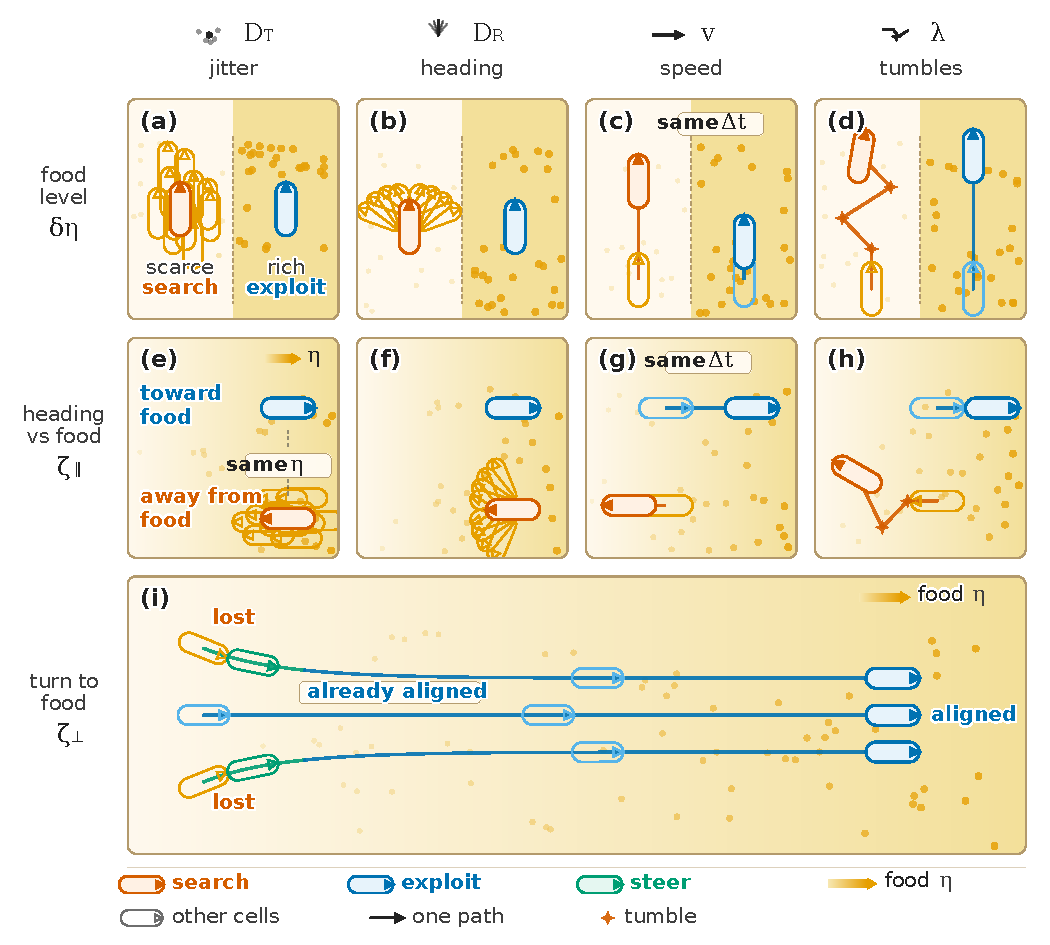
\includegraphics[width=0.70\textwidth]{figures/figure-1-response-rules.pdf}
  \caption{\textbf{Nine ways a nutrient can change how a cell moves.}  Gold
  shading is food; orange cells are in the searching state, blue in the
  exploiting state.  \emph{Rows:} what the cell reads.  Cases 1--4 (a--d) read
  only the local level $\delta\eta$---rich patch versus poor---and so cannot
  tell which way to go.  Cases 5--8 (e--h) read the alignment signal $\zp$,
  comparing a cell headed toward food with one headed away.  Case 9 (i) reads
  the transverse signal $\zeta_\perp$ and turns.  \emph{Columns:} which of the
  four motility parameters is being changed---positional jitter $D_T$, heading
  wander $D_R$, speed $v$, or tumble rate $\lambda$.  Case 8 is the classical
  \emph{E.~coli} strategy and Case 9 the eukaryotic one; see
  Table~\ref{tab:cases} for names.  Trajectories are schematic and fix the
  sign convention only.}
  \label{fig:response-rules}
\end{figure*}

\begin{figure}[tbp]
  \centering
  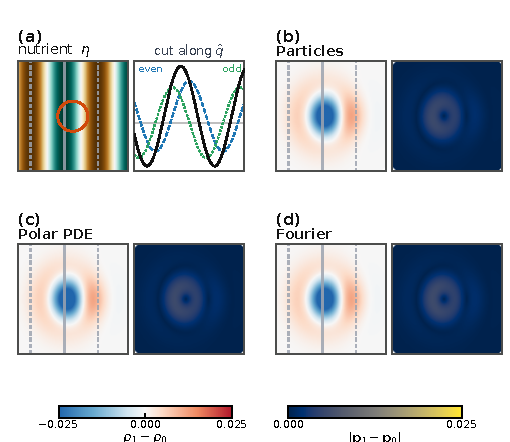
\includegraphics[width=\columnwidth]{figures/figure-3-case-1-validation.pdf}
  \caption{\textbf{The experiment, and three independent calculations of it.}
  (a) The nutrient landscape: a single cosine, with the blob of cells released
  inside the orange circle.  Solid lines mark food crests, dashed lines
  troughs, and the same marks reappear on every panel below, so the sign of a
  response can be read directly against them.  The cut along $\hat q$ shows
  why the release sits off-crest: at this phase the landscape has equal odd
  and even parts about the release point, which excites the centroid and the
  spread at the same time.  (b--d) The same problem solved three ways---by
  simulating individual cells, by integrating the coarse-grained equations,
  and by the closed-form Fourier solution---for level--jitter (Case 1) at
  $t=5\times10^{-3}$.  Each shows the density change $\rho_1-\rho_0$ beside
  the polarity change $|\mathbf p_1-\mathbf p_0|$.  \emph{What to look for:}
  the three columns should be indistinguishable, and they are, to
  $\sim1\%$.  Colour scales are shared with
  Fig.~\ref{fig:remaining-cases}; level--jitter has the weakest polarity of
  the nine, which is why those panels look nearly blank.}
  \label{fig:case1-validation}
\end{figure}

All nine live in one It\^o process for the position and heading,
\begin{subequations}
\label{eq:sde-cont}
\begin{align}
  \dd\rv_t&=v\,\ev(\theta_t)\,\dd t+\sqrt{2D_T}\,\dd\Wv_t,
  \label{eq:sde-r}\\
  \dd\theta_t&=\chi\zeta_\perp(\rv_t,\theta_t)\,\dd t
  +\sqrt{2D_R}\,\dd W_t^\theta
  +\dd\mathcal J_t^{\mathrm{tum}}
  \pmod{2\pi},
  \label{eq:sde-theta}
\end{align}
\end{subequations}
with $\Wv_t$, $W_t^\theta$ independent Wiener processes and
$\mathcal J_t^{\mathrm{tum}}$ a pure-jump process that resets the heading at
tumbles.  The corresponding Fokker--Planck equation, its no-flux wall
condition and the turning kernel are given in Appendix~\ref{app:model}.  One
detail there decides signs later: the diffusive current is $-\grad(D_TP)$,
not $-D_T\grad P$---invisible while $D_T$ is constant, decisive once the
nutrient makes it vary.

\section{From cells to two fields}
\label{sec:closure}

Tracking every cell's heading is more than any experiment reports, and more
than we need.  Three angular averages of the phase-space density $P$ carry
almost everything: the \textbf{density} $\rho$ (how many cells are here), the
\textbf{polarity} $\pv$ (which way they point, on average), and the
\emph{nematic tensor} $\Qt$ (whether they share an axis without sharing a
direction),
\begin{align}
 \rho &= \int_0^{2\pi} P\,\dd\theta,
 \qquad
 \pv = \int_0^{2\pi} \ev(\theta) P\,\dd\theta,
 \nonumber\\
 Q_{ij} &= \int_0^{2\pi} \left(n_i n_j - \tfrac12\delta_{ij}\right) P\,\dd\theta,
 \label{eq:moments}
\end{align}

Density and polarity are the two fields an imaging experiment can actually
reconstruct, so they are where we want the theory to live.

Integrating over $\theta$ gives an exact conservation law
$\partial_t\rho=-\grad\cdot\vec J^{(\rho)}$, but not a closed one: density
leans on polarity, which leans on $\Qt$, and so on up an infinite chain.  We
cut the chain at $\Qt=\mathbf0$---the \emph{polar closure}---betting that
alignment along an axis relaxes faster than transport can build it.  Three
explicit conditions control that bet (Appendix~\ref{app:closure}), and
Sec.~\ref{sec:model-comparison} measures what it costs.

The rate at which a cell forgets its heading is what sets everything below.
Rotational diffusion and tumbling both damp it, and they combine into a single
\emph{polarity relaxation rate} $\DR$ (and its nematic counterpart
$\DRtwo$),
\begin{align}
 \DR &= D_R^{(0)}+\lambda^{(0)}(1-\Pturn)>0,
 \label{eq:gamma}\\
 \DRtwo &= 4D_R^{(0)}+\lambda^{(0)}(1-\Pturntwo)>0,
 \label{eq:gamma2}
\end{align}
so $1/\DR$ is the time a cell stays pointed the same way---the natural clock
of the problem.  The nutrient shifts this rate through two combinations,
\begin{align}
 \mathcal D_R^{(\eta)} &= D_R^{(\eta)} + (1-\Pturn)\lambda^{(\eta)},
 \nonumber\\
 \mathcal D_R^{(\zp)} &= D_R^{(\zp)} + (1-\Pturn)\lambda^{(\zp)}.
 \label{eq:gamma-response}
\end{align}

These do different jobs.  $\mathcal D_R^{(\eta)}$ is a change of tempo with no
direction in it: cells forget their heading faster in richer patches, but
nothing tells them where richer patches lie.  $\mathcal D_R^{(\zp)}$ does
carry direction---it converts the alignment signal into a genuine bias along
$\grad\eta$.  With the closure in hand, the angular moments close on
\begin{subequations}
\label{eq:polar-closed-system}
\begin{align}
 \partial_t\rho &= -\grad\cdot\vec J^{(\rho)},
 \label{eq:polar-closed-density}\\
 \partial_t p_i &= -\partial_j J_{ij}^{(p)} + R_i^{(p)},
 \label{eq:polar-closed-polarity}
\end{align}
\end{subequations}
whose three constitutive pieces---the density flux, the polarity flux and the
angular source---are written out in Appendix~\ref{app:closure}.

Two patterns here drive everything below.

First, \emph{the fluxes feel only the speed and jitter rules}---level--jitter,
level--speed, aimed--jitter and aimed--speed (Cases 1, 3, 5, 7).  The four
turning rules and steering touch no flux at all; they enter through the
angular source $\vec R^{(p)}$ alone.  A turning rule can therefore move a
population only by first tilting its polarity and then waiting for that
polarity to carry cells---a detour that will cost it powers of time, and which
is the origin of the whole hierarchy in Sec.~\ref{sec:observable-hierarchy}.

Second, aimed--speed (Case 7) is exceptional twice over: it pushes density
directly, without polarizing anything first, and it alone manufactures nematic
order out of the density.

\section{The four numbers a film gives}
\label{sec:observables}

The experiment we have in mind is a \emph{release}: drop a compact blob of
cells at one point of the landscape and film it.  Few experiments resolve
$\rho$ and $\pv$ everywhere; most report a handful of numbers per frame.  This
section shows that those numbers obey closed equations of their own, and that
they suffice to identify the mechanism.  We watch only while the cloud stays
clear of the wall, $v_{\max}t+\sqrt{4D_{T,\max}t}\ll1-r_0$.

With $\vec x$ the displacement from the release point, a film of the cloud
yields four numbers per frame:
\begin{equation}
\begin{gathered}
 \Pnet=\int\pv\,\dd^2x,
 \qquad
 \Xc=\frac1N\int\vec x\,\rho\,\dd^2x,\\
 S=\frac1N\int|\vec x|^{2}\rho\,\dd^2x,
 \;\;
 T_{ij}=\frac1N\int\bigl(x_ix_j-\tfrac12|\vec x|^{2}\delta_{ij}\bigr)\rho\,\dd^2x,
\end{gathered}
 \label{eq:observable-definitions}
\end{equation}
the \emph{heading} $\Pnet$ (which way the cloud points), the \emph{centroid}
$\Xc$ (where it has moved to), the \emph{width} $S$, and the \emph{shape}
$\Tsh$ (how elongated it is, and along which axis).  Integrating
Eqs.~\eqref{eq:polar-closed-system} over the plane turns two field equations
into four ordinary differential equations for exactly these
(Appendix~\ref{app:observables}).  The nutrient enters them only through six
averages of the landscape weighted by the cloud, and through nothing else; no
gradient expansion, adiabatic elimination or weak-landscape assumption has
been made.

Two consequences are visible before any of it is solved, and both are
diagnostic.

\emph{Parity.}  A landscape that is odd about the release point---food on one
side---moves the population; an even one---a ridge or valley through the
release point---only reshapes it.  Which half of the landscape you release
into decides which of the four numbers responds at all.

\emph{No flux can create alignment.}  The speed and jitter rules enter the
equations only as fluxes, and a flux can push headings around without ever
making them.  So if a release develops a net heading, a turning rule or
steering is at work, and the speed and jitter rules are excluded outright.
That is the first entry in the readout below---and notice how much it buys for
how little: one glance at whether the cloud points anywhere cuts nine
candidates to five.

\begin{readout}
a net heading develops & a turning or steering rule; no flux rule can polarize
$\Rightarrow$ 2,\,4,\,6,\,8,\,9\\[2pt]
no heading, but the centroid moves & a speed rule $\Rightarrow$ 3,\,7\\[2pt]
neither heading nor centroid moves, ever & a jitter rule $\Rightarrow$
1,\,5\\[2pt]
only the width responds; the cloud stays round & a jitter rule again---a
gradient feeds the trace alone\\[2pt]
you released on a crest or in a valley & only width and shape can
respond; move off-centre to see the centroid\\
\end{readout}

\begin{figure*}[tp]
  \centering
  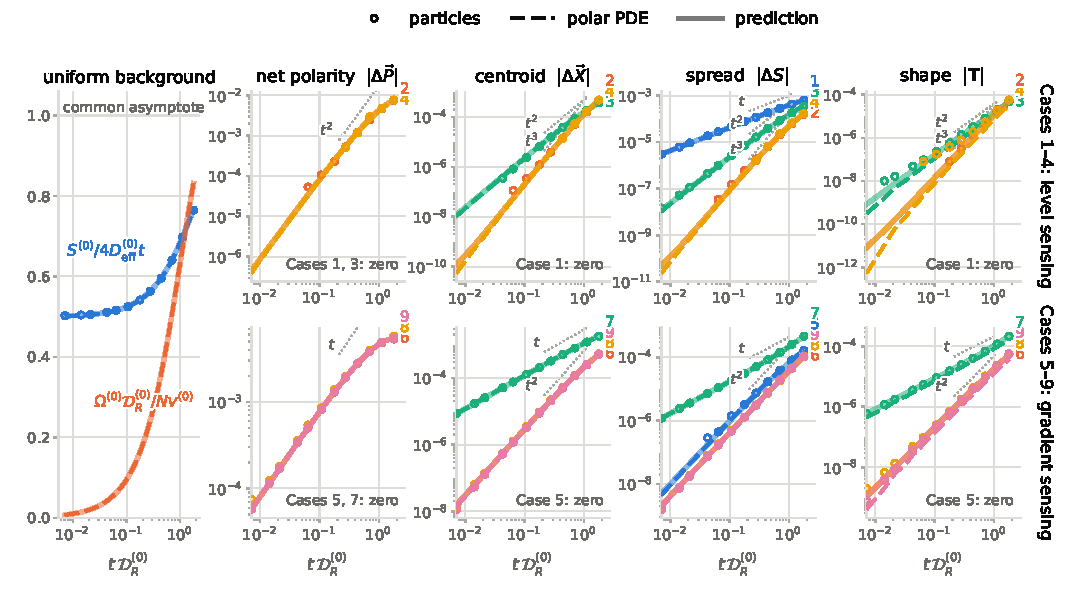
\includegraphics[width=0.98\textwidth]{figures/figure-4-macroscopic-observables.pdf}
  \caption{\textbf{Each mechanism switches on at its own time, and the slopes
  identify it.}  \emph{Left:} the uniform-landscape baseline.  The cloud
  spreads ballistically until cells forget their heading at $t\DR=1$, then
  diffusively; the outward alignment saturates at the same moment.  One such
  curve calibrates $v^{(0)}$, $D_T^{(0)}$ and $\DR$ before any nutrient is
  applied.  \emph{Right:} the response of each of the four observables, with
  the baseline subtracted, for the level rules (top row) and the aimed rules
  and steering (bottom row); curves are labelled by case number.
  \emph{What to look for:} the slope on these log--log axes is the power of
  $t$, and the dotted guides are the predictions of
  Table~\ref{tab:observable-hierarchy}---so a curve running parallel to its
  guide confirms the mechanism's signature.  Circles are simulated cells,
  dashed lines the coarse-grained solver, pale lines the closed-form theory.
  Markers are plotted only where a response exceeds twice its sampling error,
  so where a curve begins is the experimental resolution limit, not a physical
  onset.}
  \label{fig:macroscopic-observables}
\end{figure*}

\section{Timing: when each rule shows itself}
\label{sec:observable-hierarchy}

Start at the beginning of the film.  Different rules do not switch on at the
same moment, and the reason is simple:
a freshly released blob has density immediately but no polarity at all, so any
rule that must work through polarity is delayed.  Formally, the three
landscape averages weighted by density start finite, and the three weighted by
polarity start at zero and grow like $t$.

One rule then generates the whole hierarchy: \emph{the leading power of $t$ is
the power its driving overlap starts at, plus one for every time integration
between that average and the observable}.  Steering, for instance, reaches the
heading through a density-weighted average, so $\Pnet\sim t$; the heading then
drives the centroid, so $\Xc\sim t^{2}$.  Tracing each route through
Eqs.~\eqref{eq:observable-balance} gives
Table~\ref{tab:observable-hierarchy} with no further calculation.

\begin{table}[tbp]
\caption{\textbf{When each mechanism becomes visible.}  Entries are the
leading power of $t$ with which a rule's signal grows in each observable, read
off Eqs.~\eqref{eq:observable-balance}: a higher power means a later, weaker
onset and a longer film.  The four observables are the net polarity $\Pnet$
(mean heading), centroid $\Xc$ (where the cloud went), spread $S$ (how wide),
and shape $\Tsh$ (how elongated).  A dash means \emph{identically zero}, not
merely small---a structural blind spot no ensemble size repairs.  Reading the
rows: aimed--speed is the fastest to appear, level--wander and level--tumble
the slowest, and the two jitter rules are invisible in three of the four
observables.  For an idealized point release the Case 6--9 entries in $S$ and
$\Tsh$, and Case 7's in $\Tsh$, are delayed by one further power of $t$; all
other entries are release-independent.}
\label{tab:observable-hierarchy}
\begin{ruledtabular}
\begin{tabular}{@{}cl cccc@{}}
Case & Rule (sensitivity) & $\Pnet$ & $\Xc$ & $S$ & $\Tsh$\\
     &                    & heading & centroid & width & shape\\
\colrule
1 & level--jitter\ \ $D_T^{(\eta)}$ & --- & --- & $t$ & ---\\
2 & level--wander\ $D_R^{(\eta)}$ & $t^2$ & $t^3$ & $t^3$ & $t^3$\\
3 & level--speed\quad $v^{(\eta)}$ & --- & $t^2$ & $t^2$ & $t^2$\\
4 & level--tumble\ $\lambda^{(\eta)}$ & $t^2$ & $t^3$ & $t^3$ & $t^3$\\
5 & aimed--jitter\ \ $D_T^{(\zp)}$ & --- & --- & $t^2$ & ---\\
6 & aimed--wander\ $D_R^{(\zp)}$ & $t$ & $t^2$ & $t^2$ & $t^2$\\
7 & aimed--speed\quad $v^{(\zp)}$ & --- & $t$ & $t$ & $t$\\
8 & aimed--tumble\ $\lambda^{(\zp)}$ & $t$ & $t^2$ & $t^2$ & $t^2$\\
9 & steering\qquad\ \ \ $\chi$ & $t$ & $t^2$ & $t^2$ & $t^2$\\
\end{tabular}
\end{ruledtabular}
\end{table}

\textbf{Result.}  \emph{The exponents sort the nine rules into six
distinguishable groups.}  Two sets stay merged---level--wander with
level--tumble, and aimed--wander with aimed--tumble and steering---and they
are merged by the model itself, not by weak statistics: they enter only
through the combinations $\mathcal D_R^{(\eta)}$ and
$\chi-\mathcal D_R^{(\zp)}$.  No ensemble size separates them.

This is a statement about experimental design, and a sharp one.  Over a window
$t\ll1/\DR$, the level--wander signal stands to the level--jitter signal as
$\mathcal D_R^{(\eta)}(v^{(0)})^{2}t^{2}/D_T^{(\eta)}$---about one per cent
for the parameters below.  Film a release for a fifth of a heading-relaxation
time and it will tell you almost nothing about how food shifts the turning
statistics, no matter how many cells you count.  Watching longer beats
counting more.

\begin{readout}
signal grows as $t$ & aimed--speed, or level--jitter in the width alone
$\Rightarrow$ 7, 1\\[2pt]
signal grows as $t^{2}$ & the rule needs one heading relaxation first
$\Rightarrow$ 3,\,5,\,6,\,8,\,9\\[2pt]
signal appears only for $t\gtrsim1/\DR$, then as $t^{3}$ & a level turning rule
$\Rightarrow$ 2,\,4\\[2pt]
nothing yet & you may simply be early: check $t\DR$ before concluding the
response is absent\\
\end{readout}

\section{Two coefficients, not one}
\label{sec:long-time}

Wait long enough and the nine rules stop being nine.  Once $t\gg1/\DR$, every
cell has forgotten its original heading many times over; the polarity stops
leading the density and starts merely following it, and what is left is
textbook drift--diffusion,
$\partial_t\rho=\grad\cdot[D_{\mathrm{eff}}\grad\rho-\varepsilon\kappa\rho\grad\eta_1]$.
Only three numbers survive: the \emph{effective diffusivity}
$D_{\mathrm{eff}}^{(0)}=D_T^{(0)}+(v^{(0)})^{2}/2\DR$ (how fast the cloud
spreads when swimming is added to jiggling), its landscape-dependent shift
$\delta D_{\mathrm{eff}}$, and the \textbf{chemotactic mobility} $\kappa$,
\begin{equation}
 \kappa = \underbrace{\frac{v^{(0)}\bigl(\chi - \mathcal D_R^{(\zp)}\bigr)+\DR\,v^{(\zp)}}{2\DR}}_{\text{gradient responses}}
 \;-\;\underbrace{\left[D_T^{(\eta)}+\frac{v^{(0)}v^{(\eta)}}{2\DR}\right]}_{\text{level responses}} .
 \label{eq:drift-mobility}
\end{equation}

Of these, $\kappa$ is the one that decides where the cells end up: at steady
state $\rho\propto\exp[\varepsilon\kappa\eta_1/D_{\mathrm{eff}}^{(0)}]$, so
$\kappa>0$ means a heap on the food.  Notice that the level rules contribute
to it---the second bracket---and that this is no bookkeeping artefact.  It is
the traffic argument again, now with a coefficient attached: slower cells
linger, lingering cells accumulate.  In the limit of no jiggling it reduces to
the familiar $\rho\propto1/v$~\cite{schnitzer1993,tailleur2008}.

Now the trap, which is the central point of this paper.  One expects the
cloud's centre of mass to drift at $\kappa\grad\eta_1$---surely the
coefficient that says where cells end up also says how fast they head there.
It does not.  Picture a blob straddling a region where the diffusivity varies:
it spills faster to one side than the other, so its centre moves, and that
displacement has nothing to do with where the blob will eventually settle.  It
adds on top.  The centroid therefore obeys a \emph{second, different}
coefficient, the \textbf{pulse drift} $\mathcal V$,
\begin{equation}
\begin{split}
 \mathcal V={}&\frac{v^{(0)}\bigl(\chi-\mathcal D_R^{(\zp)}\bigr)
 +\DR\,v^{(\zp)}+v^{(0)}v^{(\eta)}}{2\DR}\\
 &-\frac{\bigl(v^{(0)}\bigr)^2\mathcal D_R^{(\eta)}}{2\bigl[\DR\bigr]^2},
\end{split}
 \label{eq:pulse-drift}
\end{equation}
in which the level--jitter sensitivity $D_T^{(\eta)}$ has cancelled
\emph{exactly}.  So level--jitter accumulates cells on food without ever
moving the centre of mass, and---as Sec.~\ref{sec:foraging} shows---it is also
one of the rules that feeds the population best.

The two can point opposite ways, and the cleanest example is level--speed
(Case 3): cells swim faster where food is richer.  Then $\mathcal V>0$ but
$\kappa<0$.  Early on the cloud's centre moves \emph{toward} the food, because
that is the direction it spills fastest.  Late on the population is heaped on
the \emph{poor} side, where cells crawl and dawdle.  One rule, two opposite
answers---because they answer two different questions.  ``Which way is it
going?'' and ``where does it end up?'' are not the same question, and this
paper is largely about not confusing them.

\textbf{Result.}  \emph{A measured centroid velocity is not a chemotactic
coefficient.}  Report one and call it chemotaxis, and you can be wrong about
the magnitude and about the sign.

\begin{readout}
the cloud drifts toward food & you have measured $\mathcal V$, and you do not
yet know where the cells will end up\\[2pt]
you want to know where they end up & measure the width, which gives
$\kappa$\\[2pt]
$\kappa$ and $\mathcal V$ have opposite signs & a level speed rule
$\Rightarrow$ 3\\[2pt]
$\kappa\neq0$ but $\mathcal V=0$ & level--jitter $\Rightarrow$ 1: accumulation
with no drift at all\\
\end{readout}

That said, three long-time numbers cannot carry nine rules, and waiting for
steady state throws most of the information away: level--wander and
level--tumble become indistinguishable, the three aimed-turning rules collapse
onto one mobility, and aimed--jitter vanishes from all three numbers
(Table~\ref{tab:mode-inversion}).  Recovering the rest means reading the same
film earlier (Sec.~\ref{sec:observable-hierarchy}) or one cell at a time
(Sec.~\ref{sec:information}).  What the late film \emph{does} return, and how
to read it off cleanly, is the next section.

\section{Saturation: what one release returns}
\label{sec:observable-saturation}

Two coefficients call for two measurements, and one film supplies both---but
only once it has run long enough, and only if the right two moments are read
off it.  One practical warning first.  A release in a periodic landscape does
\emph{not} drift steadily: once the cloud has spread across a wavelength the
gradient it feels averages to nothing and all motion stops, after
$\tau_\ell=1/(D_{\mathrm{eff}}^{(0)}q^{2})$.  \emph{It reports a total
displacement, not a velocity}---fitting a slope gives an answer that depends
on when filming stopped.  What it does report is
\begin{equation}
\begin{aligned}
 \Xc(\infty)&=\frac{\varepsilon\,\mathcal V}{D_{\mathrm{eff}}^{(0)}q}\,\hat q
 &&\text{(odd mode)},\\[2pt]
 \Delta S(\infty)&=-\frac{4\varepsilon\,\kappa}{D_{\mathrm{eff}}^{(0)}q^{2}}
 &&\text{(even mode)},
\end{aligned}
 \label{eq:observable-saturation}
\end{equation}
with $\Delta S=S-S^{(0)}$ the excess spread over a uniform landscape.

\textbf{Result.}  \emph{The centroid saturates on the drift; the width
saturates on the mobility.}  The two coefficients are separately readable off
one release.  The second line is worth pausing on: a population that
accumulates on food ends up \emph{narrower} than one in a uniform
landscape---concentrating on the crests is literally a reduction in width, so
measuring the width measures $\kappa$.

Better still, one parity suffices.  The width uses only the trace of the
second moment; its traceless part---the shape $\Tsh$ of
Eq.~\eqref{eq:observable-definitions}---comes from the same images at no extra
cost, and on an even mode it saturates on \emph{the drift},
\begin{equation}
 T_{\parallel}(\infty)=-\frac{2\varepsilon\,\mathcal V}
 {D_{\mathrm{eff}}^{(0)}q^{2}},
 \label{eq:shape-saturation}
\end{equation}
with $T_\parallel$ measured along $\hat q$.

\textbf{Result.}  \emph{One landscape mode returns both coefficients at once,
from the two parts of one tensor}: how wide the cloud got gives $\kappa$, how
elongated it got gives $\mathcal V$.  Where the two disagree, the population
is being pushed by a position-dependent diffusivity rather than steered, and
the size of the disagreement says how much.

Two properties make the shape the better of the two to measure.  No jitter
rule appears in it---a diffusive flux is a gradient, and a gradient feeds only
the trace---so level--jitter and aimed--jitter cannot elongate a cloud at all.
And a uniform landscape leaves the cloud exactly round, so unlike the width
the shape carries no background to subtract: the whole measured signal is
response.  Appendix~\ref{app:observables} adds the finite-width and
finite-wavenumber corrections, and the heading plateau, which supplies a third
independent combination.

\begin{readout}
final width, even mode & \emph{returns} the mobility
$\kappa=-D_{\mathrm{eff}}^{(0)}q^{2}\,\Delta S(\infty)/4\varepsilon$\\[2pt]
final elongation, even mode & \emph{returns} the drift $\mathcal V$, with no
background to subtract\\[2pt]
final centroid, odd mode & \emph{returns} $\mathcal V$ again---a
consistency check\\[2pt]
cloud stopped moving & you have waited long enough; stop filming at a few
$\tau_\ell$\\[2pt]
elongation stays zero & a jitter rule $\Rightarrow$ 1,\,5\\
\end{readout}

\begin{figure}[tbp]
  \centering
  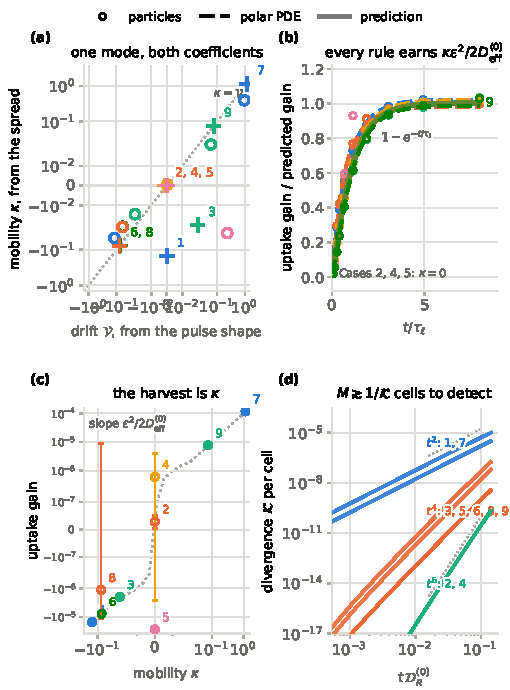
\includegraphics[width=\columnwidth]{figures/figure-5-foraging-observables.pdf}
  \caption{\textbf{What one release measures, and what the population earns by
  it.}  (a) Drift against mobility.  Reading the width and the elongation of
  the settled cloud returns $\mathcal V$ and $\kappa$ separately; circles are
  recovered values, crosses the values put in, and the dotted diagonal is
  where the two coefficients would agree.  \emph{The point of the panel is the
  points that lie off that diagonal}: level--speed (3) sits in the opposite
  quadrant---it drifts toward food while accumulating away from it---and
  level--jitter (1) sits on the vertical axis, accumulating strongly with no
  drift whatever.  (b) Uptake over time, each rule divided by its own
  predicted gain; all collapse onto $1-e^{-t/\tau_\ell}$, so a single
  landscape clock governs feeding.  (c) The harvest law itself: nutrient
  actually collected against the mobility $\kappa$ put in, falling on one
  line.  Level--wander (2) and level--tumble (4) sit at the origin and earn
  nothing.  Aimed--jitter (5) is the exception that proves the rule---it earns
  a real gain with $\kappa=0$, because it feeds at one order beyond this
  expansion.  (d) How distinguishable each rule is from a non-responding
  forager; $1/\mathcal K$ is the number of cells a detection needs, and the
  grouping is by the exponent each rule inherits.}
  \label{fig:foraging}
\end{figure}

\section{Foraging: what the population earns}
\label{sec:foraging}

Transport moments say where a population goes.  A foraging experiment asks a
different question---what does it actually eat?---and the answer turns out to
be governed by $\kappa$, not by the drift $\mathcal V$.  Define the
\textbf{uptake} $\mathcal U$ as the nutrient concentration the average cell
finds itself in,
\begin{equation}
 \mathcal U(t)=\frac1N\int\rho\,\eta\,\dd^2x .
 \label{eq:uptake-definition}
\end{equation}

The wall is impermeable, so $\mathcal U$ changes only through the flux running
along the landscape.  Once alignment is quasi-static and the landscape is
coarse compared with a run,
\begin{equation}
 \dot{\mathcal U}
 = \underbrace{D_{\mathrm{eff}}^{(0)}\bigl\langle\lap\eta\bigr\rangle}_{\text{passive}}
 \;+\;
 \underbrace{\kappa\bigl\langle|\grad\eta|^{2}\bigr\rangle}_{\text{harvest}}
 \;+\;\ord(\varepsilon^{2}).
 \label{eq:harvest-law}
\end{equation}

The two terms differ in kind.  The \emph{passive} term is what diffusion
does to any population at all: it smears cells over the landscape, erasing
whatever advantage the release point happened to offer.  It would be there for
a dead cell.  The \emph{harvest} term is what the response actually
earns---the mobility multiplied by the mean-square gradient the population
currently sits in.

\textbf{Result.}  \emph{$\kappa$ is a foraging efficiency}: nutrient collected
per unit of squared gradient available.  The same number that fixes where
cells end up also fixes how well they eat on the way.

Two cancellations deserve names.  The diffusivity shift
$\delta D_{\mathrm{eff}}$ drops out of Eq.~\eqref{eq:harvest-law}
entirely---spreading faster where food is plentiful does not, by itself, feed
anyone---yet the level--jitter sensitivity $D_T^{(\eta)}$ survives inside
$\kappa$.  This is the exact mirror of Eq.~\eqref{eq:pulse-drift}, where it
cancelled: \emph{the rule that moves no centre of mass is precisely the one
that feeds the population, and the rule that moves the centre of mass fastest
need not feed it at all.}

The sign of the gain is the sign of $\kappa$, and it reads homely.  Both
$D_T^{(\eta)}<0$ and $v^{(\eta)}<0$ give $\kappa>0$: a population profits by
\emph{slowing down and jittering less where the food is rich}---by lingering
once it finds a good patch.  That is area-restricted search, and
Eq.~\eqref{eq:harvest-law} says exactly how much it is worth.

A plate assay reports neither a rate nor a displacement but a ratio, and on
one mode of amplitude $\varepsilon$ the zero-flux state gives it in closed
form,
\begin{equation}
 \frac{\rho_{\max}}{\rho_{\min}}=e^{2\mathrm{Pe}},
 \qquad
 \mathrm{Pe}=\frac{\kappa\varepsilon}{D_{\mathrm{eff}}^{(0)}},
 \label{eq:accumulation-ratio}
\end{equation}

The \textbf{P\'eclet number} $\mathrm{Pe}$ is the only dimensionless group in
the problem, and it is the number to quote when asking whether a mechanism
matters.  It is at once the logarithm of the fold-accumulation, the fractional
density contrast a weak landscape produces, and---since drift overtakes
diffusion at $\mathrm{Pe}\simeq1$---the fractional reduction in the time a
population needs to find a target.  \emph{A rule with $|\mathrm{Pe}|\ll1$ is
biologically invisible however impressive its microscopic sensitivity looks on
paper.}  Note again which coefficient appears: a steady state carries no flux,
so $\delta D_{\mathrm{eff}}$ cancels and accumulation, like harvest, measures
$\kappa$.

Finally, a timing point that matters for how long an assay should run.  Spread
and uptake read different parts of the landscape and so run on different
clocks: the spread is set by the size of the arena, saturating after
$\tau_R=1/(D_{\mathrm{eff}}^{(0)}k_1^{2})$, while the uptake is locked to the
food patches themselves, saturating after
$\tau_\ell=1/(D_{\mathrm{eff}}^{(0)}q^{2})$.  Their ratio,
\begin{equation}
 \frac{\tau_\ell}{\tau_R}=\left(\frac{k_1\ell}{2\pi\mathcal R}\right)^{2}
 \simeq0.086\left(\frac{\ell}{\mathcal R}\right)^{2},
 \label{eq:two-clocks}
\end{equation}
is small whenever the food is patchier than the dish; for the parameters below
it is $1/186$.

\textbf{Result.}  \emph{Foraging finishes long before mixing does.}  A
population collects essentially all the nutrient available to it while its
density still looks far from steady.  Local optimization is fast, global
mixing is slow, and an assay that waits for the density to settle has waited a
couple of hundred times longer than the biology required---and has spent that
time measuring the dish rather than the cells.

\begin{readout}
uptake rate, once alignment is steady & \emph{returns} $\kappa$, independently
of the release\\[2pt]
fold-accumulation $\rho_{\max}/\rho_{\min}$ & \emph{returns} $\kappa$ once
more, as $e^{2\mathrm{Pe}}$\\[2pt]
cells accumulate but eat nothing extra & a rule with $\kappa=0$
$\Rightarrow$ 2,\,4\\[2pt]
$|\mathrm{Pe}|\ll1$ & the rule is biologically invisible, whatever its
microscopic sensitivity\\[2pt]
uptake plateaus, density still drifting & normal: the two run on clocks
$(\ell/\mathcal R)^{2}$ apart\\
\end{readout}

\begin{figure}[tbp]
  \centering
  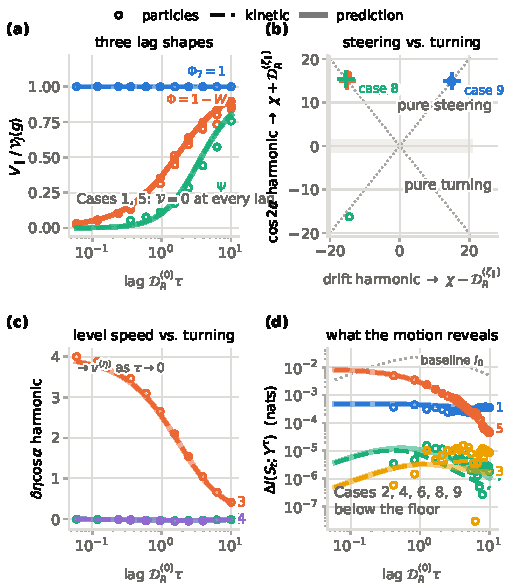
\includegraphics[width=\columnwidth]{figures/figure-6-information-observables.pdf}
  \caption{\textbf{What tracking single cells adds, and what it does not.}
  All panels use a constant gradient and a common observation lag $\tau$.
  (a) How fast a tracked cell really climbs, divided by the drift of the whole
  cloud.  Every curve saturates at one---\emph{a single cell watched long
  enough climbs at exactly the population's drift}---but reaches it through
  one of only three shapes, set by how many heading relaxations the rule needs
  before it can move a cell.  The two jitter rules (1, 5) stay flat at zero at
  every lag.  (b) Sorting the same tracks by initial heading returns two
  independent combinations, so pure steering (9) and pure turning (6, 8)
  separate---which no population measurement can do.  (c) The same trick on
  the level rules separates level--speed (3), which returns the bare
  sensitivity $v^{(\eta)}$ as the lag closes, from level--wander and
  level--tumble (2, 4), which vanish with the lag.  (d) How much a cell's
  motion reveals about its state, above the baseline that a merely swimming
  cell already provides.  \emph{Note the reversal:} the jitter rules, which
  never carry a cell up-gradient, dominate here, while the turning rules that
  navigate well sit below the estimator's floor.}
  \label{fig:information}
\end{figure}

\section{Tracking: what one cell adds}
\label{sec:information}

Everything so far uses the density and polarity at a single time.  Tracking
individual cells costs more, and buys two things a population picture cannot
supply: it separates rules the fields merge, and it pulls apart two notions
that are constantly conflated---\emph{navigating well} and \emph{moving
informatively}.

Watch one cell over a fixed \emph{lag} $\tau$, from $t$ to $t+\tau$.  Write
$g=|\grad\eta|$ for the gradient strength, $\alpha$ for the
\emph{heading error}---the angle between where the cell points and where the
food is---and $\mathcal S_t=(\rv_t,\alpha_t)$ for the cell's state relative to
the nutrient.  Every rule is then judged by one and the same random variable,
the \emph{distance made good} up the gradient the cell actually faced,
\begin{equation}
 Y^{\tau}=\bigl(\rv_{t+\tau}-\rv_t\bigr)\cdot\hat g(\rv_t).
 \label{eq:projected-displacement}
\end{equation}

Two things can be asked of $Y^\tau$.  Its average is a
\emph{navigation velocity} $V_\parallel$: how fast this cell really climbs.
Its full distribution is a \emph{communication channel}, and the mutual
information $\Irate$ it carries says how much an observer watching the cell
learns about where it started relative to the food,
\begin{equation}
 V_\parallel(t;\tau)=\frac{\mathbb E\bigl[Y^\tau\bigr]}{\tau},
 \qquad
 \Irate(t;\tau)=\frac{I\bigl(\mathcal S_t;Y^\tau\bigr)}{\tau},
 \label{eq:navigation-observables}
\end{equation}

Using the same variable for all nine rules is what puts a speed response and a
tumble response on an equal footing: no rule-specific ``controller action'' is
invented, and no coefficient is frozen during the window.

\subsection{Navigation: the same drift, on a lag clock}

Taking the release as the window start and working to first order gives,
remarkably,
\begin{equation}
 \boxed{\;V_{\parallel,j}(0;\tau)=\mathcal V_j\,\langle g\rangle\,
 \Phi_j\!\left(\DR\tau\right)\;}
 \label{eq:projected-velocity-result}
\end{equation}
with $\mathcal V_j$ the very same pulse drift as Eq.~\eqref{eq:pulse-drift},
and only three lag shapes among all nine rules,
\begin{equation}
\begin{gathered}
 W(u)=\frac{1-e^{-u}}{u},\qquad
 \Phi(u)=1-W(u)\simeq\frac u2,\\
 \Psi(u)=1-\frac{2-(2+u)e^{-u}}{u}\simeq\frac{u^{2}}{6},
\end{gathered}
 \label{eq:lag-shapes}
\end{equation}
distributed as
\begin{equation}
 \Phi_7=1,\quad
 \Phi_{3,6,8,9}=\Phi,\quad
 \Phi_{2,4}=\Psi,\quad
 \mathcal V_1=\mathcal V_5=0 .
 \label{eq:lag-hierarchy}
\end{equation}

\textbf{Result.}  \emph{Watched long enough, a tracked cell climbs at exactly
the rate the whole cloud's centre of mass drifts}---individual navigation and
pulse drift are one number.  The lag decides only how much of that rate is
visible, through one of just three curves.

Those three shapes are the short-time hierarchy again, now in the lag domain,
and the counting is once more a counting of delays.  Aimed--speed needs none:
a cell that speeds up whenever it happens to point up-gradient makes progress
on its first step.  Level--speed, aimed--wander, aimed--tumble and steering
need one---the heading must be biased before displacement follows.
Level--wander and level--tumble need two.  The jitter rules never navigate at
any lag: a diffusivity that depends on position drifts the population but not
the individual.

Sorting the windows by the cell's initial heading buys more.  The average
climb carries $\chi-\mathcal D_R^{(\zp)}$, but the $\cos2\alpha$ harmonic of
the same data carries $\chi+\mathcal D_R^{(\zp)}$.  Two independent
combinations separate genuine steering from heading-dependent turning---the
one degeneracy no population measurement can break---and it is no accident
that the missing information sits in exactly the harmonic the closure
discarded.

\subsection{Information: what the motion gives away}

At short lag the channel is Gaussian with no approximation,
$Y^\tau=\tau\mu(\mathcal S)+\sqrt{2D_T(\mathcal S)\tau}\,Z$ with
$\mu=v(\mathcal S)\cos\alpha$, so the rate follows in closed form,
\begin{equation}
 \boxed{\;\Irate(t;0^{+})=\frac{\Var[\mu(\mathcal S_t)]}{4D_T^{(0)}}
 +\frac{\Var[\delta(\mathcal S_t)]}{4\tau}\;},
 \label{eq:short-lag-information}
\end{equation}
with $\delta$ the relative change in diffusivity,
$D_T=D_T^{(0)}[1+\delta]$.  Two features of this formula do the work.

First, the baseline is already positive: $\Irate_0=(v^{(0)})^{2}/8D_T^{(0)}$
even with no sensing at all.  A cell that merely swims moves further along its
own heading than across it, so watching it tells you something about which way
it pointed.  \emph{Movement information is therefore not, by itself, evidence
of sensing}---an inference that has to be made against this baseline, not
against zero.

Second, only the rules that change the \emph{step} are legible: the two speed
rules through $\Var[\mu]$ and the two jitter rules through $\Var[\delta]$
[Eq.~\eqref{eq:information-cases}].  All four turning rules and steering leave
the rate exactly at baseline, because they change the heading before anything
has moved.  The two jitter rules are singular as well as dominant---their
channel is a scale mixture rather than a shifted Gaussian, so the total
information saturates and the \emph{rate} diverges as $\tau\to0$, which is why
a common positive lag is required for any fair comparison.  And the drift
never appears at all: shifting every outcome by the same amount tells an
observer nothing about the state.

\textbf{Result.}  \emph{Navigating well and moving informatively are
dissociated.}  The two jitter rules never carry a cell up-gradient at any lag,
yet they dominate what its motion reveals; level--wander and level--tumble
navigate perfectly well and reveal almost nothing.  The comfortable intuition
that a better forager must be a more legible one gets no support here, and an
inference method that assumes it will misread the mechanism.

\begin{readout}
climbing rate flat at zero, every lag & a jitter rule $\Rightarrow$
1,\,5\\[2pt]
climbing rate saturates at once & aimed--speed $\Rightarrow$ 7\\[2pt]
information rate diverges as $\tau\to0$ & a jitter rule again $\Rightarrow$
1,\,5\\[2pt]
information rate sits at the swimming baseline & a turning rule $\Rightarrow$
2,\,4,\,6,\,8,\,9\\[2pt]
$\cos2\alpha$ harmonic off the turning line & steering $\Rightarrow$ 9,
separated from 6 and 8\\[2pt]
$\delta\eta\cos\alpha$ harmonic finite as $\tau\to0$ & level--speed
$\Rightarrow$ 3, separated from 2 and 4\\
\end{readout}

\section{Numerical test}
\label{sec:model-comparison}

Two independent numerical descriptions test the construction: direct
simulation of the microscopic jump--diffusion, Eq.~\eqref{eq:sde-cont}, and a
conservative finite-volume integration of the closed system,
Eq.~\eqref{eq:polar-closed-system}.  All three calculations share one release,
one nutrient field and one parameter set, and no transport coefficient is
fitted.  The landscape is a single cosine of wavenumber $q\mathcal R=7.0156$
and amplitude $\varepsilon=0.25$, so every closed form above applies verbatim;
Appendix~\ref{app:numerics} explains that choice, the calibration, and the
flux discretization a chemotactic measurement is sensitive to.

Figure~\ref{fig:case1-validation} shows level--jitter (Case 1), the strictest
sign check available: cells accumulate where they jiggle \emph{least}, and a
theory that mishandles the position-dependent diffusivity gets the sign
backwards.  The three methods agree to relative $L^{2}$ density errors of
$7.2\times10^{-3}$ and $1.0\times10^{-2}$, at cosine similarities $0.99998$
and $0.99996$.

The four release observables give the sharpest test, because simulated cells
estimate them as plain averages---no binning, no bandwidth, no field to
reconstruct.  Figure~\ref{fig:macroscopic-observables} confirms three
predictions at once: the uniform background reproduces the
ballistic-to-diffusive crossover at $t\DR=1$; every response enters at the
power of $t$ Table~\ref{tab:observable-hierarchy} assigns it, with fitted
exponents within a per cent; and the structural zeros hold exactly.  The
shape $\Tsh$ is measured here for the first time, and its sharpest
prediction holds: the two jitter rules return elongations consistent with
zero ($z=1.2$ and $-0.3$), while the other seven match theory to $1.3\%$.

Figure~\ref{fig:foraging} tests the saturation and harvest laws.  Reading the
width and elongation of one settled cloud returns $\kappa$ and $\mathcal V$ to
within $2.5\%$ for every rule that has them, and every feeding rule collapses
onto $1-e^{-t/\tau_\ell}$ with a gain independent of wavelength, as
Eq.~\eqref{eq:accumulation-ratio} requires.
Figure~\ref{fig:information} tests the tracked-cell predictions against a
solution of the kinetic problem itself, since the coarse-grained fields cannot
produce a two-time law: the lag shapes, the harmonic separations and the
information baseline all come through, with the turning rules four orders of
magnitude below the two jitter rules.

Residuals are of two known kinds, and both are understood.  Simulated cells
and the coarse-grained solver differ by about a per cent on the polarity and
centroid and by up to seven on the shape---the ordering of exposure to the
discarded nematic harmonic.  The solver then departs from the first-order
theory at second order in the response amplitude: halving every sensitivity
halves the gap.  Once a response is resolved to better than a per cent, the
residual settles at the size of the neglected harmonic,
$(v^{(0)}q/\DRtwo)^{2}=3.8\%$ here---so this window is exactly where the
closure's own error becomes the limiting systematic.

\section{Discussion}
\label{sec:discussion}

Three practical messages come out of all this, and they are worth separating
from the machinery that produced them.

\emph{A centroid velocity is not a chemotactic coefficient.}  The mobility
$\kappa$, which fixes where a population ends up and how much it eats, is a
different number from the drift $\mathcal V$ that its centre of mass displays.
They can differ in magnitude, and for a speed rule they differ in sign.  Both
come off a single release---the width of the settled cloud gives one, its
elongation the other---so there is no excuse for reporting only the drift, as
chemotaxis assays routinely do.

\emph{When you look decides what you can see.}  Early on, all nine rules are
distinguishable; over an intermediate window they sort into six groups; at
steady state only three numbers survive.  An assay run to equilibrium has
thrown most of the information away, and has waited far longer than the cells
needed: feeding runs on the landscape's clock, mixing on the dish's, and here
those are a factor of $186$ apart.

\emph{A better forager is not a more informative one.}  The rules whose motion
reveals most about a cell's state are precisely the two that never carry it
up-gradient, while the best navigators sit at the baseline that mere swimming
already supplies.  Any inference scheme assuming that legibility tracks
performance will read the mechanism backwards.

Table~\ref{tab:inversion} collects the practical content of all three in one
place: each row an experiment, what it returns, and which rules it separates.

\emph{One mode, or many?}  We have worked throughout with a single sinusoid,
and that was a choice, not a restriction.  To first order in the contrast the
theory is linear in the landscape, so an arbitrary $\eta$ can be built by
superposing modes and the responses simply add.  But the reading becomes
harder, and it is worth seeing why.  Each mode saturates on its own clock,
$\tau_\ell(q)\propto q^{-2}$, and contributes to the final width and
elongation with its own $q$-dependent weight: the mobility term scales as
$q^{-2}$ while the run-length correction of
Eq.~\eqref{eq:observable-run-correction} does not.  A broadband landscape
therefore returns not $\kappa$ and $\mathcal V$ but weighted integrals of
them over the spectrum, and recovering the coefficients means deconvolving a
measured $\tilde\eta(\vec q)$---an inversion that is well posed in principle
and ill conditioned in practice, since the short-wavelength modes decay first
and contribute least.  The practical advice is the obvious one: if you can
choose the landscape, choose one wavelength, and repeat at a second to
separate the two $q$-scalings.  If you cannot---in a natural, patchy
environment---the same formulas still apply mode by mode, but expect the
answer to be a spectrum-weighted average rather than a clean coefficient.

Three approximations delimit everything above: the linear response laws, the
polar closure, and the weak-landscape and wall-free windows.  Two pairs of
rules stay merged throughout, and both are broken by the same missing
measurement---nematic order---which would also resolve the few-per-cent
closure systematic.  That is the natural next experiment.

\appendix

\section{Model, kinetic equation and boundary condition}
\label{app:model}

\subsection{Dimensionless variables}

Take $\mathcal R$ as the length scale and let the reference translational
diffusivity $\mathcal D_T^{(0)}>0$ set the time scale
$\mathcal R^2/\mathcal D_T^{(0)}$.  Then
\begin{equation}
  \rv=\frac{\vec{r}_{\mathrm{phys}}}{\mathcal R},
  \qquad
  t=\frac{\mathcal D_T^{(0)}t_{\mathrm{phys}}}{\mathcal R^2},
  \label{eq:nondimensionalization}
\end{equation}
and $\rv$ lives in the unit disk $\Ud=\{\rv\in\mathbb R^2:|\rv|<1\}$.
Everything below is dimensionless.  Speeds are measured in
$\mathcal D_T^{(0)}/\mathcal R$, translational diffusivities in
$\mathcal D_T^{(0)}$, and angular diffusivities and tumbling rates in
$\mathcal D_T^{(0)}/\mathcal R^2$, so that $D_T^{(0)}=1$.  We nonetheless keep
writing $D_T^{(0)}$ in the formulas: it keeps their dimensional origin visible
and lets them be read straight against simulation parameters.  The cell number
$N$ is left unnormalized.

A cell is a point $\rv\in\Ud$ carrying a heading angle $\theta\in[0,2\pi)$
measured from the first coordinate axis.  The heading and its perpendicular
are
\begin{equation}
\begin{split}
  \ev(\theta)&=(\cos\theta,\sin\theta)^{\mathsf T},\\
  \evp(\theta)&=(-\sin\theta,\cos\theta)^{\mathsf T},
\end{split}
\qquad
  \partial_\theta\ev=\evp,
  \quad
  \partial_\theta^2\ev=-\ev.
  \label{eq:heading-identities}
\end{equation}

\subsection{Admissibility of the linear response}

Equation~\eqref{eq:response} is a linear response law, so it makes sense only
where every speed, diffusivity and rate stays nonnegative.  A sufficient
condition is
\begin{equation}
  |X^{(\eta)}|\,\|\delta\eta\|_\infty
  +|X^{(\zp)}|\,\|\grad\eta\|_\infty\leq X^{(0)},
  \label{eq:admissible}
\end{equation}
for each $X$, with $\|\cdot\|_\infty$ the largest magnitude over $\Ud$.  This
marks where the linearization holds; it is not a saturation law.  Check the
two terms separately, because a gentle nutrient contrast does not guarantee a
gentle gradient.  The Fokker--Planck problem below needs one thing more,
$D_T>0$, or the spatial equation degenerates.  Steering is bounded on its own
by $|\chi|\,\|\grad\eta\|_\infty/\DR\ll1$, with $\DR$ the reference
polarity-relaxation rate of Eq.~\eqref{eq:gamma}.

\subsection{The stochastic process and the wall}

Here $\Wv_t$ is a two-dimensional standard Wiener process, $W_t^\theta$ an
independent scalar one, and every coefficient is evaluated at the current
state through Eq.~\eqref{eq:response}.  The pure-jump process
$\mathcal J_t^{\mathrm{tum}}$ stays constant between tumbles; at a tumble it
resets the heading from $\theta_{t^-}$ to $\theta_{t^+}$ and leaves the
position alone.

Two short-time relations fix the normalization of the diffusivities.  Hold the
coefficients fixed over $\Delta t$: the translational noise then produces a
mean-square displacement $4D_T\Delta t$, and the rotational noise an angular
variance $2D_R\Delta t$.

The wall stops cells without turning them: a displacement that would leave
$\Ud$ loses its outward normal component and the cell slides along the
boundary on what is left, heading untouched.  This normal-constraint
(Skorokhod) reflection becomes the no-flux condition
Eq.~\eqref{eq:microscopic-no-flux} in phase space, imposed for every heading
separately.  Because the heading is untouched, a cell pressed into the wall
stays pressed until it turns away, and a polarity layer builds along the
boundary.  Every result below lives inside the wall-free window of
Sec.~\ref{sec:observables}, where no cell reaches the wall at all, so we
state the rule and then never use it.

\subsection{Tumble rate and turning law}

Tumbling needs two ingredients: the rate $\lambda(\rv,\theta)$ says when a
cell tumbles, and the normalized kernel $\mathcal T(\theta'\mid\theta)$ says where it
points afterwards.  Both are evaluated at the pre-tumble state.  For a
rotationally invariant, achiral kernel,
\begin{equation}
\begin{gathered}
  \mathcal T(\theta'\mid\theta) = \widehat{\mathcal T}(\Delta\theta),\qquad
  \widehat{\mathcal T}(\Delta\theta) = \widehat{\mathcal T}(-\Delta\theta),\\
  \int_0^{2\pi}\mathcal T(\theta'\mid\theta)\,\dd\theta'=1,
\end{gathered}
  \label{eq:turning-symmetry}
\end{equation}
where $\Delta\theta=\theta'-\theta\pmod{2\pi}$.  The one number we need from
this kernel is its first harmonic,
\begin{equation}
  \Pturn = \int_0^{2\pi}\cos(\Delta\theta)\,\widehat{\mathcal T}(\Delta\theta)\,\dd(\Delta\theta),
  \quad -1 \leq \Pturn \leq 1,
  \label{eq:turn-persistence}
\end{equation}
the mean heading a tumble retains: $\Pturn=1$, $0$ and $-1$ are a forward run,
a uniform reorientation and a U-turn.  Achirality kills the transverse mean,
so a tumble does nothing but damp alignment, contributing
$\lambda^{(0)}(1-\Pturn)$ to the polarity-relaxation rate below.

\subsection{Fokker--Planck master equation}

Let $P(\rv,\theta,t)$ be the number density on the phase space
$\Ud\times\mathbb S^1$, so that
\begin{equation}
  \int_{\Ud}\int_0^{2\pi}P(\rv,\theta,t)\,\dd\theta\,\dd^2r=N,
  \label{eq:total-number}
\end{equation}
with initial data $P(\rv,\theta,0)=P_0$ nonnegative, normalized to $N$,
$2\pi$-periodic, and compatible with no flux at the wall.

The It\^o process of Eq.~\eqref{eq:sde-cont} carries spatial and angular
currents
\begin{equation}
  \vec J_{\mathrm{sp}}=v\ev P-\grad(D_TP),
  \qquad
  J_{\mathrm{ang}}=\chi\zeta_\perp P
  -\partial_\theta(D_RP),
  \label{eq:phase-currents}
\end{equation}
and the Fokker--Planck master equation
\begin{align}
  \partial_tP={}&-\grad\cdot\vec J_{\mathrm{sp}}
   -\partial_\theta J_{\mathrm{ang}}
  \nonumber\\
  &+\int_0^{2\pi}\lambda(\rv,\theta')\mathcal T(\theta\mid\theta')
  P(\rv,\theta',t)\,\dd\theta'
  \nonumber\\
  &-\lambda(\rv,\theta)P(\rv,\theta,t).
  \label{eq:kinetic}
\end{align}
The gain term uses the source rate $\lambda(\rv,\theta')$, and normalization
of $T$ balances gain against loss.  One detail deserves a flag now, because it
decides signs later: the spatial diffusive current is $-\grad(D_TP)$, not
$-D_T\grad P$.  The difference is invisible while $D_T$ is constant and
decisive the moment the nutrient makes it vary.

Two boundary conditions close the problem.  The wall is impermeable, so the
normal spatial current vanishes for every heading,
\begin{equation}
  \nv\cdot\vec J_{\mathrm{sp}}=0
  \qquad \rv\in\partial\Ud,\quad\theta\in[0,2\pi),
  \label{eq:microscopic-no-flux}
\end{equation}
with $\nv$ the outward unit normal.  The heading is an angle, so $P$ and
$J_{\mathrm{ang}}$ are $2\pi$-periodic in $\theta$.  Integrating
Eq.~\eqref{eq:kinetic} over the whole phase space then kills all three
contributions in turn---the wall term by Eq.~\eqref{eq:microscopic-no-flux},
the angular term by periodicity, the tumble term by normalization of
$\mathcal T$---and leaves $N$ exactly conserved.

\section{The polar closure and its validity}
\label{app:closure}

The exact density flux, before any closure, is
\begin{align}
 \vec J^{(\rho)} ={}& (v^{(0)}+v^{(\eta)}\delta\eta)\pv
 + v^{(\zp)}\left(\tfrac12\rho\Id + \mathbf Q\right)\grad\eta
 \nonumber\\
 & - \grad\left[(D_T^{(0)}+D_T^{(\eta)}\delta\eta)\rho
 + D_T^{(\zp)}\pv\cdot\grad\eta\right].
 \label{eq:exact-flux}
\end{align}

Setting $\Qt=\mathbf0$ requires three conditions.  First, the population must
stay near-isotropic,
\begin{equation}
  \frac{2|\pv|}{\rho} \ll 1.
  \label{eq:near-isotropy-condition}
\end{equation}
Second, on the scale $L_\eta$ over which the landscape varies, transport must
be slow compared with nematic decay,
\begin{equation}
  \frac{v^{(0)}}{\DRtwo L_\eta} \ll 1.
  \label{eq:polar-closure-validity}
\end{equation}
Third, Case 7 needs a condition of its own.  Take the traceless second
angular moment of Eq.~\eqref{eq:kinetic} and keep the isotropic part of the
fourth moment.  At $\pv=\vec0$ exactly one nutrient source of $\mathbf Q$
survives, the Case-7 term
\begin{equation}
 \Sigma_{ij} = -\frac{v^{(\zp)}}{8}\Bigl[\partial_i(\rho\,\partial_j\eta)
 +\partial_j(\rho\,\partial_i\eta)
 -\delta_{ij}\grad\cdot(\rho\grad\eta)\Bigr];
 \label{eq:case7-nematic-source}
\end{equation}
where every other rule reaches $\mathbf Q$ only through $\pv$.  Balancing
$\Sigma_{ij}$ against relaxation at $\DRtwo$ and imposing $2|\mathbf Q|/\rho\ll1$
gives
\begin{equation}
  \frac{|v^{(\zp)}|}{\DRtwo}
  \left(\|\nabla\nabla\eta\|_\infty+\frac{\|\grad\eta\|_\infty}{L_\rho}\right)
  \ll 1,
  \label{eq:case7-nematic-validity}
\end{equation}
with $\|\nabla\nabla\eta\|_\infty$ the largest Hessian magnitude over the
sampled region and $L_\rho$ the scale on which the density varies.  Both terms
matter: expanding $\partial_i(\rho\partial_j\eta)$ gives
$\rho\,\partial_i\partial_j\eta$ and $\partial_i\rho\,\partial_j\eta$, and
whenever the density varies on the landscape's own scale the second is as
large as the first.

The three constitutive pieces of Eqs.~\eqref{eq:polar-closed-system} are
\begin{align}
 \vec J^{(\rho)} ={}& (v^{(0)}+v^{(\eta)}\delta\eta)\pv
 + \frac{v^{(\zp)}\rho}{2}\grad\eta
 \nonumber\\
 & - \grad\left[(D_T^{(0)}+D_T^{(\eta)}\delta\eta)\rho
 + D_T^{(\zp)}\pv\cdot\grad\eta\right],
 \label{eq:polar-closed-density-flux}\\
 J_{ij}^{(p)} ={}& \frac{\rho}{2}(v^{(0)}+v^{(\eta)}\delta\eta)\delta_{ij}
 \nonumber\\
 & + \frac{v^{(\zp)}}{4}\left[
 p_i\partial_j\eta + p_j\partial_i\eta + (\pv\cdot\grad\eta)\delta_{ij}\right]
 \nonumber\\
 & - \partial_j\left[(D_T^{(0)}+D_T^{(\eta)}\delta\eta)p_i
 + \frac{D_T^{(\zp)}\rho}{2}\partial_i\eta\right],
 \label{eq:polar-closed-polarity-flux}\\
 \vec R^{(p)} ={}& -\left[\DR+\mathcal D_R^{(\eta)}\delta\eta\right]\pv
 + \frac{(\chi - \mathcal D_R^{(\zp)})\rho}{2}\grad\eta,
 \label{eq:polar-closed-angular-source}
\end{align}

\section{Uniform background and the weak landscape}
\label{app:propagator}

\subsection{Wall-free window and the plane limit}

On the plane the system is linear and translationally invariant, so it has a
Green propagator: the density and polarity produced at $(\rv,t)$ by a point
release at $(\rv',t')$, depending only on $\rv-\rv'$ and $t-t'$.

That one object does two jobs.  Convolved with an arbitrary initial profile it
gives the uniform-background evolution.  Convolved instead---through Duhamel's
principle---with the forcing a weak landscape spreads through space, it gives
the first-order population response.

\subsection{Spectrum and Green propagator}
\label{sec:uniform-spectrum}

For $\eta=\eta^{(0)}$ ($\delta\eta=0$, $\grad\eta=\vec0$),
Eqs.~\eqref{eq:polar-closed-system} collapse to
\begin{subequations}
\label{eq:uniform-density-polarity}
\begin{align}
 \partial_t\rho&=D_T^{(0)}\lap\rho-v^{(0)}\grad\cdot\pv,
 \label{eq:uniform-density}\\
 \partial_t\pv&=D_T^{(0)}\lap\pv-\DR\pv
 -\frac{v^{(0)}}{2}\grad\rho.
 \label{eq:uniform-polarity}
\end{align}
\end{subequations}
Read these two lines physically: translational diffusion acts equally on both
fields, the speed $v^{(0)}$ couples density gradients to polarity flux and
back, and alignment relaxes isotropically at $\DR$.  With the convention
$\tilde f(\vec k)=\int e^{-i\vec k\cdot\rv}f\,\dd^2r$, so that
$\grad\to i\vec k$ and $\lap\to-k^2$, decompose the polarity relative to
$\hat{\vec k}=\vec k/k$,
\begin{equation}
 \tilde\pv = \tilde p_L\,\hat{\vec k} + \tilde p_T\,\hat{\vec k}_{\perp},
 \qquad \hat{\vec k}_{\perp}=(-\hat k_2,\hat k_1)^{\mathsf T}.
 \label{eq:polarity-fourier-decomposition}
\end{equation}
Gradients and divergences act strictly along $\vec k$, so the transverse
polarity generates no spatial flux and feels no density coupling.  It simply
decays,
\begin{equation}
 \tilde p_T(\vec k,t) = \tilde p_{T,0}(\vec k)\,e^{-\left(D_T^{(0)}k^2+\DR\right)t}.
 \label{eq:arbitrary-transverse-solution}
\end{equation}
Density and longitudinal polarity form a coupled pair,
$\partial_t(\tilde\rho,\tilde p_L)^{\mathsf T}
=\mathbf M(k)(\tilde\rho,\tilde p_L)^{\mathsf T}$, with
\begin{equation}
 \mathbf M(k) = \begin{pmatrix}
   -D_T^{(0)}k^2 & -i v^{(0)}k \\
   -\frac{i v^{(0)}k}{2} & -\left(D_T^{(0)}k^2 + \DR\right)
 \end{pmatrix}.
 \label{eq:longitudinal-system-matrix}
\end{equation}
Define the mean damping and spectral splitting
\begin{equation}
 \mu_k = \tfrac12\operatorname{Tr}(-\mathbf M) = D_T^{(0)}k^2 + \tfrac12\DR
 \label{eq:mean-damping-rate}
\end{equation}
and the traceless remainder $\mathbf A(k)$, whose square is a multiple of the
identity, $\mathbf A^2=(\sigma_k/2)^2\Id$, with the spectral splitting
\begin{equation}
 \sigma_k = \sqrt{\bigl[\DR\bigr]^2 - 2\bigl[v^{(0)}\bigr]^2 k^2}.
 \label{eq:longitudinal-spectral-scales}
\end{equation}
The longitudinal propagator $\mathbf G_L(k,t)=e^{\mathbf M(k)t}$ is
\begin{widetext}
\begin{equation}
 \mathbf G_L(k,t)
 =e^{-\mu_kt}
 \begin{pmatrix}
 \displaystyle
 \cosh\!\left(\frac{\sigma_kt}{2}\right)
 +\frac{\DR}{\sigma_k}
 \sinh\!\left(\frac{\sigma_kt}{2}\right)
 &\displaystyle
 -\frac{2iv^{(0)}k}{\sigma_k}
 \sinh\!\left(\frac{\sigma_kt}{2}\right)
 \\
 \displaystyle
 -\frac{iv^{(0)}k}{\sigma_k}
 \sinh\!\left(\frac{\sigma_kt}{2}\right)
 &\displaystyle
 \cosh\!\left(\frac{\sigma_kt}{2}\right)
 -\frac{\DR}{\sigma_k}
 \sinh\!\left(\frac{\sigma_kt}{2}\right)
 \end{pmatrix},
 \label{eq:longitudinal-green-matrix}
\end{equation}
\end{widetext}
acting on any initial $(\tilde\rho_0,\tilde p_{L,0})^{\mathsf T}$.  Together
with Eq.~\eqref{eq:arbitrary-transverse-solution} this is the complete
uniform-background dynamics---no approximation, no fitting.

The sign of $\sigma_k^2$ splits the behaviour into two regimes.  For
$k<k_c=\DR/(\sqrt2v^{(0)})$ the splitting $\sigma_k$ is real and the
longitudinal modes decay at the two rates $\mu_k\mp\sigma_k/2$, which as
$k\to0$ become
\begin{align}
 s_{\text{slow}}(k) &= \left(D_T^{(0)} + \frac{(v^{(0)})^2}{2\DR}\right)k^2 + \ord(k^4), \label{eq:slow-diffusive-mode}\\
 s_{\text{fast}}(k) &= \DR + \left(D_T^{(0)} - \frac{(v^{(0)})^2}{2\DR}\right)k^2 + \ord(k^4). \label{eq:fast-relaxing-mode}
\end{align}
On macroscopic scales density therefore decays diffusively with the enhanced
diffusivity
Eq.~\eqref{eq:macroscopic-effective-diffusivity}
the familiar enhancement of diffusion by self-propulsion, while polarity
mismatches relax at $\DR$.

Above $k_c$ the splitting turns imaginary and the hyperbolic functions become
trigonometric, $\cosh(\sigma_kt/2)\to\cos(|\sigma_k|t/2)$ and
$\sigma_k^{-1}\sinh(\sigma_kt/2)\to|\sigma_k|^{-1}\sin(|\sigma_k|t/2)$.
Spatial gradients then drive transient polar-advection waves at frequency
$\omega_k=|\sigma_k|/2$ under the envelope $e^{-\mu_kt}$.  The wavenumber
$k_c$ is where long-range macro-diffusion gives way to short-range transient
waves: cells cross a wavelength before they forget their heading.

\subsection{Point release}
\label{sec:dirac-homogeneous}

For a centered release of $N$ cells with isotropic headings,
$P(\rv,\theta,0)=(N/2\pi)\delta^{(2)}(\rv)$, i.e.
$\rho_0=N\delta^{(2)}(\rv)$ and $\pv_0=\vec0$, the Fourier initial data are
$\tilde\rho_0=N$, $\tilde p_{L,0}=0$, and
Eq.~\eqref{eq:longitudinal-green-matrix} gives
\begin{equation}
 \tilde\rho^{(0)}(k,t) = N A_k(t), \qquad \tilde p_i^{(0)}(\vec k,t) = -i N \hat{k}_i\, B_k(t),
 \label{eq:dirac-reference-fourier-fields}
\end{equation}
with the per-cell Green amplitudes
\begin{subequations}
\label{eq:dirac-amplitudes}
\begin{align}
 A_k(t) &= e^{-\mu_k t}\left[\cosh\left(\frac{\sigma_k t}{2}\right) + \frac{\DR}{\sigma_k}\sinh\left(\frac{\sigma_k t}{2}\right)\right],
 \label{eq:dirac-density-amplitude}\\
 B_k(t) &= e^{-\mu_k t}\frac{v^{(0)}k}{\sigma_k}\sinh\left(\frac{\sigma_k t}{2}\right).
 \label{eq:dirac-polarity-amplitude}
\end{align}
\end{subequations}
Both amplitudes have plain readings.  $A_k$ follows the pulse as it broadens,
carrying it from ballistic spreading at short times to isotropic diffusion at
long ones.  $B_k$ follows the radial polarity that builds up while cells
stream away from the release point, and that fades once their headings
decorrelate.

The source is isotropic, so the real-space fields follow from
inverse Hankel transforms,
\begin{subequations}
\label{eq:dirac-hankel-transforms}
\begin{align}
 \rho^{(0)}(r,t) &= \frac{N}{2\pi}\int_0^\infty k\,\dd k\,J_0(kr) A_k(t),
 \label{eq:dirac-density-hankel}\\
 p_r^{(0)}(r,t) &= \frac{N}{2\pi}\int_0^\infty k\,\dd k\,J_1(kr) B_k(t).
 \label{eq:dirac-polarity-hankel}
\end{align}
\end{subequations}
Equations~\eqref{eq:dirac-amplitudes} and \eqref{eq:dirac-hankel-transforms}
carry single-cell dynamics straight onto the population propagator.  Five
single-cell numbers, $(v^{(0)},D_T^{(0)},D_R^{(0)},\lambda^{(0)},\Pturn)$, fix
the entire spatial evolution.  Nothing is left to fit.

\subsection{Duhamel expansion and the first-order kernels}

Let the landscape be weak and static,
\begin{equation}
 \eta(\rv) = \eta^{(0)} + \varepsilon \eta_1(\rv), \qquad 0 < \varepsilon \ll 1,
 \label{eq:weak-nutrient-field}
\end{equation}
and expand $\rho=\rho^{(0)}+\varepsilon\rho^{(1)}+\ord(\varepsilon^2)$ and
$\pv=\pv^{(0)}+\varepsilon\pv^{(1)}+\ord(\varepsilon^2)$.  The initial data
stay fixed, so the corrections start from nothing,
$\rho^{(1)}(\rv,0)=0$ and $\pv^{(1)}(\rv,0)=\vec0$, and $(\rho^{(0)},\pv^{(0)})$
is exactly the uniform-background evolution of App.~\ref{app:propagator}.

At $\ord(\varepsilon)$ the coupling is a convolution: a nutrient mode at
$\vec k'$ meets a population mode at $\vec k-\vec k'$ and produces a response
at $\vec k$.  Three kernels carry it---one for the density flux, one for the
polarity flux, one for the angular source---and all nine microscopic rules
live in them, and nowhere else.  Their explicit forms, and the effective
forcings $\tilde f_\rho$ and $\tilde f_{p,i}$ obtained by integrating them
against the nutrient spectrum $\tilde\eta_1(\vec k')$, are collected in
Eqs.~\eqref{eq:weak-density-flux}--\eqref{eq:weak-polarity-forcing} below.
What matters here is their structure, and it is the structure that drives
everything below: a response acts either on $\tilde\rho^{(0)}$ or on
$\tilde\pv^{(0)}$, and it enters either a flux or the polarity source.

Explicitly,
\begin{widetext}
\begin{align}
 \tilde J_{\rho,i}^{(1)}(\vec k,\vec k',t')
 ={}&v^{(\eta)}\tilde p_i^{(0)}
 +\frac{i v^{(\zp)}}{2}\tilde\rho^{(0)} k'_i
 -iD_T^{(\eta)}\tilde\rho^{(0)} k_i
 +D_T^{(\zp)}\left[\tilde\pv^{(0)}\cdot\vec k'\right] k_i,
 \label{eq:weak-density-flux}\\
 \tilde J_{ij}^{(p)(1)}(\vec k,\vec k',t')
 ={}&\frac{v^{(\eta)}}{2}\tilde\rho^{(0)}\delta_{ij}
 +\frac{i v^{(\zp)}}{4}\left[
 \tilde p_i^{(0)} k'_j
 + k'_i\,\tilde p_j^{(0)}
 +\left(\tilde\pv^{(0)}\cdot\vec k'\right)\delta_{ij}
 \right]
 -iD_T^{(\eta)}\tilde p_i^{(0)} k_j
 +\frac{D_T^{(\zp)}}{2}\tilde\rho^{(0)} k'_i k_j,
 \label{eq:weak-polarity-flux}\\
 \tilde R_{p,i}^{(1)}(\vec k,\vec k',t')
 ={}&-\mathcal D_R^{(\eta)}\tilde p_i^{(0)}
 +\frac{i(\chi - \mathcal D_R^{(\zp)})}{2}\tilde\rho^{(0)} k'_i,
 \label{eq:weak-polarity-source}
\end{align}
with every zeroth-order field evaluated at $(\vec k-\vec k',t')$.
Integrating them against the nutrient spectrum gives the effective forcings
\begin{align}
 \tilde f_\rho(\vec k,t')
 ={}&\int_{\mathbb R^2}\frac{\dd^2k'}{(2\pi)^2}\tilde\eta_1(\vec k')\left[-i k_i \tilde J_{\rho,i}^{(1)}(\vec k,\vec k',t')\right],
 \label{eq:weak-density-forcing}\\
 \tilde f_{p,i}(\vec k,t')
 ={}&\int_{\mathbb R^2}\frac{\dd^2k'}{(2\pi)^2}\tilde\eta_1(\vec k')\left[-i \tilde J_{ij}^{(p)(1)}(\vec k,\vec k',t') k_j + \tilde R_{p,i}^{(1)}(\vec k,\vec k',t')\right],
 \label{eq:weak-polarity-forcing}
\end{align}
\end{widetext}

which enter Eq.~\eqref{eq:weak-field-solution}.

Write $\tilde f_L=\hat k_i\tilde f_{p,i}$ and
$\tilde f_T=\hat k_{\perp,i}\tilde f_{p,i}$ for the longitudinal and
transverse projections of the polarity forcing.  By Duhamel's principle the
first-order fields are then the convolution of that forcing with the
unperturbed propagator,
\begin{subequations}
\label{eq:weak-field-solution}
\begin{align}
 \begin{pmatrix}\tilde\rho^{(1)}\\\tilde p_L^{(1)}\end{pmatrix}(\vec k,t)
 ={}&\int_0^t\mathbf G_L(k,t-t')\begin{pmatrix}\tilde f_\rho\\\tilde f_L\end{pmatrix}(\vec k,t')\,\dd t',
 \label{eq:weak-longitudinal-solution}\\
 \tilde p_T^{(1)}(\vec k,t)
 ={}&\int_0^t e^{-\left[D_T^{(0)}k^2+\DR\right](t-t')}\tilde f_T(\vec k,t')\,\dd t'.
 \label{eq:weak-transverse-solution}
\end{align}
\end{subequations}
Equation~\eqref{eq:weak-field-solution} completes the wall-free solution.  Every correction is an explicit convolution
with the measured nutrient spectrum $\tilde\eta_1(\vec k')$: no mode of the
landscape has been coarse-grained away, and a landscape given as data can be
used as data.  Specializing to the point release of
Sec.~\ref{sec:dirac-homogeneous} costs one substitution,
\begin{equation}
 \tilde\rho^{(0)}=N A_{|\Delta\vec k|}(t'),
 \quad
 \tilde p_i^{(0)}=-iN\frac{\Delta k_i}{|\Delta\vec k|}B_{|\Delta\vec k|}(t'),
 \label{eq:dirac-substitution}
\end{equation}
with $\Delta\vec k=\vec k-\vec k'$, into the kernels.  The
physical fields then follow from two-dimensional inverse transforms of
$\tilde\rho$ and $\tilde p_i$: once the landscape breaks rotational symmetry
the Hankel reduction no longer applies.  At zero wavevector, conservation and
Eq.~\eqref{eq:polar-closed-polarity} give $\tilde\rho(\vec0,t)=N$ and
$\tilde p_i(\vec0,t)=\varepsilon\int_0^te^{-\DR(t-t')}\tilde f_{p,i}(\vec0,t')\,\dd t'+\ord(\varepsilon^2)$.

\subsection{Counting the transient exponents}
\label{sec:transient-hierarchy}

The Duhamel integral has a second use.  Read at short times, it sorts the
nine rules by how far each one sits from the observable, and the counting is
easy to follow.

A release starts with density but no polarity:
$\tilde\rho^{(0)}=N+\ord(t)$ and $\tilde p^{(0)}=\ord(t)$
[Eq.~\eqref{eq:dirac-amplitudes}], and the off-diagonal blocks of
$\mathbf G_L$ are themselves $\ord(t)$.  So a response term pays one power of
$t$ for the Duhamel integration itself, a second if it multiplies $\pv^{(0)}$
rather than $\rho^{(0)}$, and a third if it enters the polarity equation
rather than the density flux.  The tally is
\begin{equation}
\begin{aligned}
 \delta\rho&\sim t:\ \{1,7\};
 \quad t^2:\ \{3,5,6,8,9\};
 \quad t^3:\ \{2,4\},\\
 \delta\pv&\sim t:\ \{3,5,6,8,9\};
 \quad t^2:\ \{1,2,4,7\}.
\end{aligned}
 \label{eq:transient-hierarchy}
\end{equation}
Only two rules move density at first order in time, and they are the two that
act on the density flux through $\rho$ itself: $D_T^{(\eta)}$ and
$v^{(\zp)}$.  Cases 2 and 4 sit farthest away.  They modulate the decay of a
polarity that must be built before it can decay, and each of those steps costs
a power of $t$.

This is a statement about experimental design, not only about asymptotics.
Over a window $t\ll1/\DR$ the Case-2 density response stands to the Case-1
response as $\mathcal D_R^{(\eta)}(v^{(0)})^2t^2/D_T^{(\eta)}$, up to a
numerical factor; for the parameters of Sec.~\ref{sec:model-comparison} that
ratio is $1.2\times10^{-2}$.

A release watched for a fifth of an orientational relaxation time therefore
says almost nothing about how the nutrient level shifts the turning
statistics---however many cells are tracked.  Seeing Cases 2 and 4 in density
needs $t\gtrsim1/\DR$, which is precisely where the fast mode of
Eq.~\eqref{eq:fast-relaxing-mode} has died and the long-time reduction below
takes over.  Section~\ref{sec:model-comparison} bears this out: at unchanged
ensemble size the two carry a thirtieth of the Case-1 density response at
$t\DR\simeq0.36$ and more than half of it at $t\DR\simeq1.78$.  Their polarity
signature arrives one power of $t$ sooner, and is the better thing to watch
early.

The enhanced diffusivity of the uniform background is
\begin{equation}
\begin{split}
 D_{\mathrm{eff}}^{(0)} &= D_T^{(0)} + \frac{(v^{(0)})^2}{2\DR}\\
 &= D_T^{(0)} + \frac{(v^{(0)})^2}{2\left[D_R^{(0)}+\lambda^{(0)}(1-\Pturn)\right]},
\end{split}
 \label{eq:macroscopic-effective-diffusivity}
\end{equation}
and the landscape shifts it by
\begin{equation}
 \delta D_{\mathrm{eff}}(\rv) = \left[ D_T^{(\eta)} + \frac{v^{(0)}v^{(\eta)}}{\DR} - \frac{(v^{(0)})^2 \mathcal D_R^{(\eta)}}{2[\DR]^2} \right] \eta_1(\rv),
 \label{eq:diffusivity-spectral-shift-explicit}
\end{equation}

\section{Long-time reduction and mode inversion}
\label{app:longtime}

\begin{table}[tbp]
\caption{\textbf{What survives at long times---and what is lost.}  After many
heading relaxations the nine rules compress onto only three measurable
numbers: a shift in how fast headings relax, a shift in the spreading rate
$\delta D_{\rm eff}$, and the mobility $\kappa$ that sets accumulation.  A
dash means no leading-order contribution.  \emph{Read the columns for the
degeneracies}: level--wander and level--tumble (2, 4) enter identically, the
three aimed-turning rules (6, 8, 9) enter only through $\kappa$, and
aimed--jitter (5) vanishes from all three---so waiting for steady state
destroys most of the information.  Here $\bar P=1-\Pturn$, and the pulse drift
is $\mathcal V=\kappa+\delta D_{\mathrm{eff}}'$.}
\label{tab:mode-inversion}
\footnotesize
\begin{ruledtabular}
\begin{tabular}{clccc}
Case & Sensitivity & $1/\tau_{\rm fast}-\DR$ & $\delta D_{\rm eff}$ & $\kappa$\\
\colrule
1 & $D_T^{(\eta)}$ & --- & $D_T^{(\eta)}$ & $-D_T^{(\eta)}$\\
2 & $D_R^{(\eta)}$ & $D_R^{(\eta)}$ & $-\frac{(v^{(0)})^2D_R^{(\eta)}}{2[\DR]^2}$ & ---\\
3 & $v^{(\eta)}$ & --- & $\frac{v^{(0)}v^{(\eta)}}{\DR}$ & $-\frac{v^{(0)}v^{(\eta)}}{2\DR}$\\
4 & $\lambda^{(\eta)}$ & $\bar P\lambda^{(\eta)}$ & $-\frac{(v^{(0)})^2\bar P\lambda^{(\eta)}}{2[\DR]^2}$ & ---\\
5 & $D_T^{(\zp)}$ & --- & --- & ---\\
6 & $D_R^{(\zp)}$ & --- & --- & $-\frac{v^{(0)}D_R^{(\zp)}}{2\DR}$\\
7 & $v^{(\zp)}$ & --- & --- & $\frac{v^{(\zp)}}{2}$\\
8 & $\lambda^{(\zp)}$ & --- & --- & $-\frac{v^{(0)}\bar P\lambda^{(\zp)}}{2\DR}$\\
9 & $\chi$ & --- & --- & $\frac{v^{(0)}\chi}{2\DR}$\\
\end{tabular}
\end{ruledtabular}
\end{table}

At long times ($t\gg1/\DR$) and long wavelengths the fast polarity mode has
died and only the slow branch is left.  Polarity then follows the density
instead of leading it: setting $\partial_t\pv=\vec 0$ in
Eq.~\eqref{eq:polar-closed-polarity} and keeping the leading spatial gradients
gives the adiabatic polarity
\begin{equation}
 \pv=\frac{1}{\mathcal D_R}\left[-\grad\!\left(\frac{\rho v}{2}\right)
 +\bigl(\chi-\mathcal D_R^{(\zp)}\bigr)\frac{\rho}{2}\grad\eta\right],
 \label{eq:adiabatic-polarity}
\end{equation}
in which $v=v^{(0)}+v^{(\eta)}\delta\eta$ and
$\mathcal D_R=\DR+\mathcal D_R^{(\eta)}\delta\eta$ still carry their landscape
dependence.  Substituting this into
Eq.~\eqref{eq:polar-closed-density-flux} collapses the density dynamics to
ordinary drift--diffusion,
\begin{equation}
 \partial_t\rho=\grad\cdot\left[D_{\mathrm{eff}}(\rv)\grad\rho
 -\varepsilon\,\kappa\,\rho\,\grad\eta_1\right],
 \label{eq:long-time-drift-diffusion}
\end{equation}
with a locally shifted diffusivity
$D_{\mathrm{eff}}(\rv)=D_{\mathrm{eff}}^{(0)}+\varepsilon\,\delta D_{\mathrm{eff}}(\rv)$,
Eq.~\eqref{eq:diffusivity-spectral-shift-explicit}
and a single chemotactic mobility
Eq.~\eqref{eq:drift-mobility}
This is the leading term of a joint expansion in $\varepsilon$ and in spatial
gradients; every term it keeps carries two spatial derivatives in all.  Case 5
first contributes at fourth order, through
$-\varepsilon D_T^{(\zp)}v^{(0)}\lap(\grad\rho\cdot\grad\eta_1)/2\DR$, which
is why $D_T^{(\zp)}$ appears in none of the coefficients below.  It will
reappear in Sec.~\ref{sec:observable-saturation}.

The second bracket of Eq.~\eqref{eq:drift-mobility} is easy to miss and not
optional.  A level response makes the transport coefficients themselves
functions of position, and a spatially varying diffusivity or speed moves
density with no directional sensing whatever.  In the It\^o convention the
flux $-\grad(D_T\rho)$ contains the drift $-\rho\grad D_T$, and eliminating
$\pv$ adiabatically supplies the companion term $-\rho\grad(v^2)/(4\DR)$.
With translational diffusion negligible this is the classical run--tumble
accumulation $\rho\propto1/v$ of a population whose speed depends on
position~\cite{schnitzer1993,tailleur2008}: cells linger where they are slow.

In a bounded domain the zero-flux state of
Eq.~\eqref{eq:long-time-drift-diffusion} is
$\rho\propto\exp[\varepsilon\kappa\eta_1/D_{\mathrm{eff}}^{(0)}]$ to
$\ord(\varepsilon)$.  So $\kappa$ is the mobility that decides where the
population ends up.

One caution before reading observables off
Eq.~\eqref{eq:long-time-drift-diffusion}: its coefficients are not constant.
$D_{\mathrm{eff}}$ varies at the same order $\varepsilon$ as the drift, so
freezing it is not innocent.

The safe route is through the two lowest moments, which are exact to
$\ord(\varepsilon)$ and are what a release experiment actually reports.
Writing $\vec x$ for the displacement from the release point and
$\langle\cdot\rangle$ for the density-weighted average,
\begin{equation}
\begin{aligned}
 \frac{\dd\langle\vec x\rangle}{\dd t}
 &=\varepsilon\,\mathcal V\,\langle\grad\eta_1\rangle,
 \qquad \mathcal V=\kappa+\delta D_{\mathrm{eff}}',\\
 \frac{\dd}{\dd t}\bigl\langle|\vec x-\langle\vec x\rangle|^2\bigr\rangle
 &=4\langle D_{\mathrm{eff}}\rangle+\ord(\varepsilon^2),
\end{aligned}
 \label{eq:pulse-moments}
\end{equation}
where $\delta D_{\mathrm{eff}}'$ is the bracket of
Eq.~\eqref{eq:diffusivity-spectral-shift-explicit}, so that
$\delta D_{\mathrm{eff}}=\delta D_{\mathrm{eff}}'\,\eta_1$.

The centroid velocity is therefore \emph{not} $\kappa\grad\eta_1$.  A
spatially varying diffusivity displaces the centroid on its own, through
$\langle\grad D_{\mathrm{eff}}\rangle$, and that displacement simply adds.
Explicitly,
Eq.~\eqref{eq:pulse-drift}
in which $D_T^{(\eta)}$ has cancelled exactly.  A pulse spreading in a
linearly varying It\^o diffusivity does not move its centroid---even though
that same response is what sets the accumulation.

The distinction is physical, not bookkeeping, and the two coefficients can
even come with opposite signs.  Take a pure speed response (Case 3) with
$v^{(\eta)}>0$, so that $\kappa<0$ while $\mathcal V>0$.  Early on the pulse
centroid moves \emph{toward} high nutrient, simply because cells spread faster
on that side.  Late on the population piles up where cells are slow, as
$\rho\propto1/v$ demands.  One rule, two directions, two different questions.

Three structural facts follow.  All three level responses set the spreading
rate, and two of them, $D_T^{(\eta)}$ and $v^{(\eta)}$, also set part of the
mobility $\kappa$---with weights that differ from their weights in
$\delta D_{\mathrm{eff}}$.  The gradient responses
($v^{(\zp)},\mathcal D_R^{(\zp)},\chi$) enter $\kappa$ alone.  And Case 5,
$D_T^{(\zp)}$, enters nothing at all at this order, by the gradient counting
above, even though it does shape the transient fields.

\subsection{Validity window}

What we have built is a Green function of the polar-closed equations for
$t>0$, not a controlled approximation to the microscopic dynamics at the
singular instant $t=0$.  Comparison with a particle simulation therefore holds
only for times and Fourier modes satisfying
\begin{equation}
\begin{gathered}
 v_{\max}t+\sqrt{4D_{T,\max}t}\ll d_{\rm wall},\\
 \frac{v^{(0)} k}{\DRtwo}\ll1,
 \qquad
 \frac{2|\pv|}{\rho}\ll1,
\end{gathered}
 \label{eq:dirac-validity-window}
\end{equation}
with $d_{\rm wall}$ the smallest distance from the initial support to the
boundary, and the last condition evaluated where the fields are compared.
Each inequality answers for one approximation: the first keeps the wall out,
the second excludes scales on which the neglected nematic harmonic is not
small, the third checks near-isotropy.

Inside this window the theory predicts the fields with no fitted transport
coefficient, so any discrepancy that survives numerical refinement is a
verdict on the closure itself.  Outside it, the wall or the higher angular
moments must be restored before a comparison means anything at all.

\subsection{Reading parameters off the mode time constants (DDM)}
\label{sec:mode-inversion}

Everything above is measurable, and the density half of it without tracking a
single cell.  Fourier-transforming a density field and watching each mode
decay is exactly what differential dynamic microscopy does: it pulls the
intermediate scattering function
$f(k,t)=\langle e^{i\vec k\cdot(\rv_t-\rv_0)}\rangle$ out of the fluctuations
of ordinary time-lapse images, averaged over $\sim10^{4}$
cells~\cite{wilson2011,martinez2012}.  Within the polar closure that function
\emph{is} the density amplitude $A_k(t)$ of
Eq.~\eqref{eq:dirac-amplitudes}.

This section runs the measurement backwards: from a decay curve to the
microscopic combination behind it.

In a uniform landscape three decay channels are available at each $k$.  The
transverse polarity decays as a single exponential with
\begin{equation}
 \tau_T(k) = \frac{1}{D_T^{(0)}k^2+\DR},
 \label{eq:tau-transverse}
\end{equation}
while for $k<k_c$ the coupled density and longitudinal polarity decay as a sum
of two exponentials,
\begin{equation}
 \tau_{\text{slow}}(k)=\frac{1}{\mu_k-\sigma_k/2}, \qquad
 \tau_{\text{fast}}(k)=\frac{1}{\mu_k+\sigma_k/2}.
 \label{eq:tau-slow-fast}
\end{equation}
For $k>k_c$ the two merge into a single decay $\mu_k$ modulated at frequency
$\omega_k=|\sigma_k|/2$, so $k_c$ shows up directly as the wavenumber where
relaxational modes give way to oscillatory ones.

Together these curves determine $(v^{(0)},D_T^{(0)},\DR)$, with one relation
to spare.  Their $k=0$ intercept fixes $\DR$; the slope of $1/\tau_T$ against
$k^2$ fixes $D_T^{(0)}$; and $v^{(0)}$ follows from
\begin{equation}
 \frac1{\tau_T(k)}-\frac1{\tau_{\text{fast}}(k)}
 \;\longrightarrow\; \frac{(v^{(0)})^2}{2\DR}\,k^2
 \qquad (k\to0),
 \label{eq:v0-extraction}
\end{equation}
the slow channel providing the cross-check through
$1/\tau_{\text{slow}}\to D_{\mathrm{eff}}^{(0)}k^2$.  These are precisely the
quantities a two-exponential fit to $f(k,t)$ returns, so the
uniform-background part of the inversion asks for no new instrument.

One decomposition is out of reach here.  Density and polarity cannot split
$\DR=D_R^{(0)}+\lambda^{(0)}(1-\Pturn)$ into its two pieces, because both
enter it the same way.  The nematic rate $\DRtwo$ can, since rotational
diffusion damps harmonic $n$ as $n^2$ while tumbling contributes
$1-\mathcal P_{n,\mathrm{turn}}$.  For the wrapped-normal kernel used here and
$\Pturn=0.3$, level-dependent rotational diffusion and tumbling drive the
second harmonic in a ratio close to $3:1$.

Repeating the release in the landscape adds three scalars: the fast-rate shift,
\begin{equation}
 \frac1{\tau_{\text{fast}}}-\DR
 \to \varepsilon\,\mathcal D_R^{(\eta)}\eta_1(\rv),
 \label{eq:mode-inversion-fast}
\end{equation}
the spreading rate $4\langle D_{\mathrm{eff}}\rangle$, and the centroid
velocity $\varepsilon\mathcal V\grad\eta_1$.  Between them these return
$(\mathcal D_R^{(\eta)},\delta D_{\mathrm{eff}},\kappa)$, with
$\kappa=\mathcal V-\delta D_{\mathrm{eff}}'$.

Table~\ref{tab:mode-inversion} shows what is left over.  Cases 2 and 4 share
the relaxation shift, Cases 6--9 share the mobility, and Case 5 is missing
altogether.  Three numbers cannot carry nine rules; separating them needs
either independent landscape components or an observable beyond density and
polarity.  The next two sections supply both.

\section{Balance laws in detail}
\label{app:observables}

\subsection{Solving for the six combinations}
\label{app:inversion-algebra}

\begin{table}[tbp]
\caption{\textbf{A field guide: which measurement identifies which
mechanism.}  This is the paper's practical summary---each row is an experiment
you can do, what it returns, and which rules it tells apart.  The first block
needs only time-lapse images of cell density, no tracking.  The second needs
the release watched until it stops changing.  The third needs single-cell
trajectories over a common lag.  \emph{Read together, the rows determine all
six combinations of Eq.~\eqref{eq:inversion-basis}, and hence all nine
sensitivities}---except two pairs (level--wander with level--tumble,
aimed--wander with aimed--tumble) that only a measurement of nematic order can
split.}
\label{tab:inversion}
\footnotesize
\begin{ruledtabular}
\begin{tabular}{@{}p{0.40\columnwidth} p{0.30\columnwidth} l@{}}
Measurement & Returns & Rules it isolates\\
\colrule
\multicolumn{3}{l}{\emph{Density images alone}}\\
Decay of $f(k,t)$, uniform background (DDM) & $v^{(0)},D_T^{(0)},\DR$ & ---\\
Shift of the fast decay rate & level turning strength & 2, 4\\
Centroid displacement, odd mode & $\mathcal V$ & ---\\
Pulse shape $T_\parallel$, even mode & $\mathcal V$ (no background) & ---\\
Spread $\Delta S$, even mode & $\kappa$ & ---\\
Spread, wavenumber-independent part & $\ell_{\mathrm{run}}v^{(\zp)}+2D_T^{(\zp)}$ & 5, 7\\
Heading plateau, with the centroid & the speed rules' share of $\mathcal V$ & 3, 7\\
Short-time exponents of $\Pnet,\Xc,S$ & which overlap drives each & six groups\\
\colrule
\multicolumn{3}{l}{\emph{Population averages over the landscape}}\\
Uptake rate $\dot{\mathcal U}$ & $\kappa$ & ---\\
Steady accumulation $\rho_{\max}/\rho_{\min}$ & $\kappa/D_{\mathrm{eff}}^{(0)}$ & ---\\
Divergence $\mathcal K$ from a null forager & squares of the above & detection cost\\
\colrule
\multicolumn{3}{l}{\emph{Tracked windows of common lag $\tau$}}\\
Projected velocity $V_\parallel(\tau)$ & $\mathcal V_j$, and $\Phi_j$ & 7 $|$ 3,6,8,9 $|$ 2,4\\
$\cos2\alpha$ harmonic & $\chi+\mathcal D_R^{(\zp)}$ & 9 from 6, 8\\
$\delta\eta\cos\alpha$ harmonic & $v^{(\eta)}$, $\mathcal D_R^{(\eta)}$ & 3 from 2, 4\\
Information rate $\Irate(\tau)$ & $(v^{(\eta)})^2,(v^{(\zp)})^2$ & 3, 7\\
Information rate as $\tau\to0$ & $(D_T^{(\eta)})^2,(D_T^{(\zp)})^2$ & 1, 5\\
\end{tabular}
\end{ruledtabular}
\end{table}


Six independent combinations exhaust what the nine rules can express.  Four
collect the contribution of one response channel each,
\begin{equation}
\begin{gathered}
 m_\chi=\frac{v^{(0)}\bigl(\chi-\mathcal D_R^{(\zp)}\bigr)}{2\DR},
 \qquad
 m_v^{(\zp)}=\frac{v^{(\zp)}}{2},\\[2pt]
 m_v^{(\eta)}=\frac{v^{(0)}v^{(\eta)}}{2\DR},
 \qquad
 m_R^{(\eta)}=\frac{\bigl(v^{(0)}\bigr)^{2}\mathcal D_R^{(\eta)}}{2\bigl[\DR\bigr]^{2}},
\end{gathered}
 \label{eq:inversion-basis}
\end{equation}
together with the two jitter sensitivities $D_T^{(\eta)}$ and $D_T^{(\zp)}$.
In this basis the transport coefficients are simple sums,
\begin{equation}
\begin{aligned}
 \mathcal V&=m_\chi+m_v^{(\zp)}+m_v^{(\eta)}-m_R^{(\eta)},\\
 \kappa&=m_\chi+m_v^{(\zp)}-m_v^{(\eta)}-D_T^{(\eta)},\\
 \mathcal V_v&=m_v^{(\zp)}+m_v^{(\eta)} ,
\end{aligned}
 \label{eq:inversion-combinations}
\end{equation}
with $\mathcal V_v$ the part of the drift carried by the two speed rules.
Reading down Table~\ref{tab:inversion} solves for all six in order.  The shift
in the fast decay rate gives $m_R^{(\eta)}$.  The polarity plateau read against
the centroid gives $\mathcal V_v$, and hence
$m_\chi=\mathcal V+m_R^{(\eta)}-\mathcal V_v$.  The short-time exponents---or
equivalently the tracked-cell lag shapes---split $m_v^{(\zp)}$ from
$m_v^{(\eta)}$.  The width gives $D_T^{(\eta)}$, and the part of it that does
not scale with wavelength gives $D_T^{(\zp)}$.

The four numbers of Eq.~\eqref{eq:observable-definitions} close on one more,
the outward polarity $\Omega=\int\vec x\cdot\pv\,\dd^2x$---how strongly cells
point away from the release point, and the only channel by which swimming
feeds spreading.  Every flux in Eqs.~\eqref{eq:polar-closed-system} is a
divergence, so inside the wall-free window it integrates away, leaving
\begin{subequations}
\label{eq:observable-balance}
\begin{align}
 \dot\Pnet&=-\DR\Pnet
 +\frac{\chi-\mathcal D_R^{(\zp)}}{2}\,\Gv
 -\mathcal D_R^{(\eta)}\Piv,
 \label{eq:observable-polarity}\\
 \dot\Omega&=-\DR\Omega+Nv^{(0)}
 +v^{(\eta)}\Erho+v^{(\zp)}\Gp
 \nonumber\\&\quad
 -\mathcal D_R^{(\eta)}\Cp
 +\frac{\chi-\mathcal D_R^{(\zp)}}{2}\,\Crho,
 \label{eq:observable-outward}\\
 N\dot\Xc&=v^{(0)}\Pnet+v^{(\eta)}\Piv+\frac{v^{(\zp)}}{2}\Gv,
 \label{eq:observable-centroid}\\
 N\dot S&=4ND_T^{(0)}+2v^{(0)}\Omega
 \nonumber\\&\quad
 +2v^{(\eta)}\Cp+v^{(\zp)}\Crho+4D_T^{(\eta)}\Erho+4D_T^{(\zp)}\Gp .
 \label{eq:observable-spread}
\end{align}
\end{subequations}

The six overlaps are named for the field they weight ($\rho$ or $\pv$) and
what they read---the level $\mathcal E$, the gradient $\mathcal G$, or the
gradient moment about the release point $\mathcal C$:
\begin{equation}
\begin{aligned}
 \Erho&=\int\rho\,\delta\eta, &\quad \Gv&=\int\rho\,\grad\eta,\\
 \Piv&=\int\delta\eta\,\pv, &\quad \Gp&=\int\pv\cdot\grad\eta,\\
 \Crho&=\int\rho\,\vec x\cdot\grad\eta, &\quad \Cp&=\int\delta\eta\,(\vec x\cdot\pv).
\end{aligned}
 \label{eq:observable-overlaps}
\end{equation}

Those taken against the density start finite; those taken against the polarity
start at zero and grow like $t$, which is the origin of the hierarchy in
Table~\ref{tab:observable-hierarchy}.

\subsection{Uniform background}

Set $\varepsilon=0$ and every overlap vanishes.  Then $\Pnet$ and $\Xc$ stay
zero by symmetry, and the remaining pair integrates in closed form,
\begin{equation}
\begin{aligned}
 \Omega^{(0)}&=\frac{Nv^{(0)}}{\DR}\left(1-e^{-\DR t}\right),\\
 S^{(0)}(t)-S(0)&=4D_T^{(0)}t\\
 &\quad+\frac{2\bigl(v^{(0)}\bigr)^{2}}{\bigl[\DR\bigr]^{2}}
 \left(\DR t-1+e^{-\DR t}\right).
\end{aligned}
 \label{eq:baseline-observables}
\end{equation}
Outward alignment saturates at $Nv^{(0)}/\DR$ within one orientational time,
and at the same moment the spread crosses over from
$4D_T^{(0)}t+\bigl(v^{(0)}t\bigr)^2$ to
$4D_{\mathrm{eff}}^{(0)}t-2\bigl(v^{(0)}\bigr)^2/[\DR]^2$: ballistic, then
diffusive.  One spreading curve therefore fixes $D_T^{(0)}$, $v^{(0)}$ and
$\DR$ before any landscape is applied---a useful calibration to have in hand.

\subsection{Saturation, refinements and the polarity plateau}

Take a single landscape mode of wavevector $\vec q$.  Its overlaps collapse
straight onto the Green amplitudes of Eq.~\eqref{eq:dirac-amplitudes}.  For an
odd mode $\varepsilon\sin(\vec q\cdot\vec x)$ about the point release of
Sec.~\ref{sec:dirac-homogeneous}, $\Gv=N\hat q\,qA_q(t)$ and
$\Piv=N\hat q\,B_q(t)$ with $\Erho=\Crho=\Cp=\Gp=0$; an even mode does the reverse; and a
release of finite width multiplies both by its own transform.

Now $A_q$ and $B_q$ are combinations of $e^{-t/\tau_{\rm slow}(q)}$ and
$e^{-t/\tau_{\rm fast}(q)}$, and
\begin{equation}
 \int_0^te^{-\DR(t-t')}e^{-st'}\dd t'
 =\frac{e^{-st}-e^{-\DR t}}{\DR-s},
 \label{eq:observable-convolution}
\end{equation}
so every observable is a fixed combination of three exponentials, at rates
already tabulated in Sec.~\ref{sec:mode-inversion}.  The macroscopic
observables bring no time scale of their own.

Two of those rates matter.  Alignment equilibrates at $\DR$.  The mode itself
then decays at $1/\tau_q=D_{\mathrm{eff}}^{(0)}q^{2}$, because once the pulse
has spread across a wavelength the gradient it feels averages away.

This has a practical consequence.  A release in a structured landscape reports
a \emph{displacement}, not a velocity: there is no slope to fit.  What it
reports is the integral of Eqs.~\eqref{eq:observable-balance} over the whole
life of the mode,
Eq.~\eqref{eq:observable-saturation}
with $\Delta S=S-S^{(0)}$.  This is the section's central result:
\emph{the centroid saturates on the drift, the spread saturates on the
mobility}.

Section~\ref{sec:long-time} argued that $\mathcal V$ and
$\kappa$ are different coefficients answering different questions.  Here one
release returns both, from two landscape components of opposite parity, and
their difference is $\delta D_{\mathrm{eff}}'$.  The second line also says
something one might not have guessed: a population that accumulates
up-gradient ($\kappa>0$) ends up \emph{narrower} than it would in a uniform
landscape, by exactly four times the accumulation length
$\kappa/D_{\mathrm{eff}}^{(0)}q^{2}$.

Neither expression needs the adiabatic elimination that produced
Eq.~\eqref{eq:pulse-moments}.  Integrating
$\dot\Pnet=-\DR\Pnet+(\text{source})$ from zero to infinity gives
$\int\Pnet\,\dd t=\int(\text{source})\dd t/\DR$ whatever the transient does,
and likewise for $\Omega$; Eq.~\eqref{eq:observable-saturation} is exact at
$\ord(\varepsilon)$.

The same integral supplies two refinements, and each carries information
rather than merely correcting a number.  First, a release of width $\sigma_0$
in a landscape of finite wavenumber replaces $1/D_{\mathrm{eff}}^{(0)}$ by
$e^{-q^{2}\sigma_0^{2}/2}/D_{\mathrm{eff}}(q)$ with
\begin{equation}
 D_{\mathrm{eff}}(q)=D_T^{(0)}
 +\frac{\bigl(v^{(0)}\bigr)^{2}}{2\bigl(D_T^{(0)}q^{2}+\DR\bigr)},
 \label{eq:mode-effective-diffusivity}
\end{equation}
the zero-frequency transfer of the propagator itself.  Second, the spread
carries a term that the gradient expansion behind
Eq.~\eqref{eq:long-time-drift-diffusion} throws away,
\begin{equation}
 \Delta S_\parallel(\infty)=-\frac{\varepsilon\,\ell_{\mathrm{run}}}{D_{\mathrm{eff}}^{(0)}}
 \left[\ell_{\mathrm{run}}\,v^{(\zp)}+2D_T^{(\zp)}\right],
 \quad \ell_{\mathrm{run}}=\frac{v^{(0)}}{\DR},
 \label{eq:observable-run-correction}
\end{equation}
smaller than the mobility term by $(q\ell_{\mathrm{run}})^{2}$ and carried \emph{only} by
the two directional flux responses.  It is the one long-time observable Case 5
reaches at all.  The two terms are cleanly separable because the mobility term
scales as $q^{-2}$ and this one does not: repeat the release at two
wavelengths and read off both.

The net polarity does not saturate.  It rises over $1/\DR$ to a quasi-static
plateau and then decays with the mode,
\begin{equation}
 \frac{\Pnet}{N}\simeq\frac{\varepsilon q}{v^{(0)}}
 \bigl[\mathcal V-\mathcal V_v\bigr]e^{-t/\tau_q}\,\hat q,
 \qquad
 \mathcal V_v=\frac{v^{(\zp)}}{2}+\frac{v^{(0)}v^{(\eta)}}{2\DR},
 \label{eq:observable-polarity-plateau}
\end{equation}
where $\mathcal V_v$ is the part of the drift carried by the two speed
responses.  Alignment thus reports the drift \emph{minus} the speed channel,
which makes sense: a rule that moves density merely by making cells faster on
one side never creates net alignment.

Reading the polarity plateau against the centroid displacement therefore
isolates $\mathcal V_v$, and Table~\ref{tab:observable-hierarchy} already
splits its two members by their exponents.  Three curves, four coefficients:
$\mathcal V$, $\kappa$, $\mathcal V_v$, and the directional pair of
Eq.~\eqref{eq:observable-run-correction}.

\subsection{Balance laws for the shape}

The traceless part $\Tsh$ of the second moment,
Eq.~\eqref{eq:observable-definitions}, is the elongation of the released
cloud, and it costs nothing extra to measure.  Repeating the integration by
parts with this traceless weight gives one more pair of balance laws,
\begin{subequations}
\label{eq:shape-balance}
\begin{align}
 N\dot T_{ij}&=v^{(0)}\hat\Omega_{ij}+v^{(\eta)}\hat{\mathcal C}_{p,ij}
 +\tfrac12 v^{(\zp)}\hat{\mathcal C}_{\rho,ij},
 \label{eq:shape-moment}\\
 \dot{\hat\Omega}_{ij}&=-\DR\hat\Omega_{ij}
 +\tfrac12v^{(\zp)}\hat{\mathcal G}_{p,ij}
 -\mathcal D_R^{(\eta)}\hat{\mathcal C}_{p,ij}
 \nonumber\\&\quad
 +\tfrac12\bigl(\chi-\mathcal D_R^{(\zp)}\bigr)\hat{\mathcal C}_{\rho,ij},
 \label{eq:shape-polarity}
\end{align}
\end{subequations}
in which $\hat\Omega_{ij}$ is the traceless outward-polarity moment and
$\hat{\mathcal C}_\rho$, $\hat{\mathcal C}_p$, $\hat{\mathcal G}_p$ are the
traceless companions of $\Crho$, $\Cp$ and $\Gp$,
obtained by replacing $x_i\partial_j\eta$ with
$x_i\partial_j\eta+x_j\partial_i\eta-\delta_{ij}\vec x\cdot\grad\eta$, and so
on.

Two things follow at once.  \emph{No translational-diffusivity response
appears.}  A diffusive flux is a gradient, and a gradient feeds only the
trace, so Cases 1 and 5 cannot shape a pulse at all.  And the uniform
background is exactly isotropic, so $\Tsh\equiv\vec0$ at $\varepsilon=0$:
unlike $S$, the shape has no background to subtract, and the whole measured
signal is the response.

What drives the shape is the anisotropy of the landscape's curvature: for a
compact release,
$\hat{\mathcal C}_{\rho,ij}\simeq\tfrac12\langle|\vec x|^2\rangle
(\partial_i\partial_j\eta-\tfrac12\delta_{ij}\lap\eta)$
evaluated at the release point.  A landscape whose Hessian happens to be
isotropic there gives no shape signal whatever its gradient.  So this
observable asks for a release where the curvature has a direction---which is
exactly what a single plane-wave mode provides.

On the even mode of Sec.~\ref{sec:observable-saturation} the shape saturates on
\emph{the drift},
Eq.~\eqref{eq:shape-saturation}
with $T_\parallel$ the component along $\hat q$---exactly half of
Eq.~\eqref{eq:observable-saturation} with $-\kappa$ replaced by $\mathcal V$.

So one even landscape mode returns both coefficients at once, from the two
parts of a single tensor: the trace gives $\kappa$, the traceless part gives
$\mathcal V$, and no mode of the opposite parity is needed.  Where the two
disagree, the population is being pushed by a spatially varying diffusivity
rather than steered.

\section{Foraging and information: details}
\label{app:information}

\subsection{One landscape mode}

On a single mode, $\eta=\eta^{(0)}+\varepsilon\cos(\vec q\cdot\vec x+\varphi)$, the harvest
law closes.  There $\langle\lap\eta\rangle=-q^{2}(\mathcal U-\eta^{(0)})$
exactly, and $\langle|\grad\eta|^{2}\rangle\to\varepsilon^{2}q^{2}/2$ once the pulse has
spread across a wavelength, so $\mathcal U$ relaxes as a single exponential
from whatever the release point offered to
\begin{equation}
 \mathcal U(\infty)-\eta^{(0)}=\frac{\kappa\varepsilon^{2}}{2D_{\mathrm{eff}}^{(0)}},
 \qquad
 \tau_\ell=\frac{1}{D_{\mathrm{eff}}^{(0)}q^{2}}=\frac{\ell^{2}}{4\pi^{2}D_{\mathrm{eff}}^{(0)}}.
 \label{eq:uptake-saturation}
\end{equation}
The two halves come apart usefully.  The gain does not depend on $q$ at all:
a fine landscape and a coarse one of the same contrast are worth the same.
The time needed to collect it does depend on $q$, as $\ell^{2}$.  A
fine-grained landscape is not richer, only quicker.

\subsection{Telling two strategies apart}

Suppose two mechanisms---or one mechanism and a null forager---produce
densities $\rho_i$ and $\rho_j$.  How hard are they to tell apart?  The
natural measure is the Kullback--Leibler divergence per cell,
\begin{equation}
 \mathcal K_{ij}=\frac1N\int\rho_i\ln\frac{\rho_i}{\rho_j}\,\dd^2x
 =\frac{1}{2N}\int\frac{(\rho_i-\rho_j)^{2}}{\rho^{(0)}}\,\dd^2x
 +\ord(\varepsilon^{3}),
 \label{eq:discrimination}
\end{equation}
the linear term vanishing because both distributions carry the same mass.
Everything now follows from one fact: $\mathcal K$ is quadratic where the
fields are linear.

Every exponent therefore doubles.  A rule whose density response grows as
$t^{n}$ in Eq.~\eqref{eq:transient-hierarchy} becomes distinguishable as
$t^{2n}$.  And $M$ independently tracked cells accumulate a log-likelihood
ratio $M\mathcal K$, so a detection needs
\begin{equation}
 M\gtrsim\mathcal K^{-1}\sim t^{-2n}.
 \label{eq:sample-size}
\end{equation}
That is the sampling floor of Sec.~\ref{sec:model-comparison} in closed form,
and it settles the experimental trade.  At fixed cost $Mt$ the evidence grows
as $t^{2n-1}$, so watching longer always beats tracking more.  For Cases 2 and
4, where $n=3$, doubling the window is worth $32$ times the cells.

The same expression states the degeneracies exactly.  Cases 2 and 4 generate
identical fields, so $\mathcal K_{24}=0$ at every time and every ensemble
size.  Cases 6, 8 and 9 generate collinear fields, differing only by the
scalar $\chi-\mathcal D_R^{(\zp)}$, so no release can separate the mechanism
from its amplitude.  Neither statement is about statistical power; both are
about the model.

\subsection{The backward generator}

Both follow from the backward generator adjoint to
Eq.~\eqref{eq:kinetic},
\begin{align}
 \mathcal Lf={}&v\,\ev\cdot\grad f+D_T\lap f
 +\chi\zeta_\perp\partial_\theta f+D_R\partial_\theta^2f
 \nonumber\\
 &+\lambda\!\int_0^{2\pi}\!\!\widehat{\mathcal T}(\Delta\theta)
 \bigl[f(\rv,\theta+\Delta\theta)-f(\rv,\theta)\bigr]\dd(\Delta\theta),
 \label{eq:backward-generator}
\end{align}
in which a state-dependent It\^o diffusivity multiplies $\lap f$, where in
the forward equation it sat inside $\lap(D_TP)$.  That difference is not
bookkeeping.  Population redistribution and single-trajectory drift are
different statements, and the two translational-diffusivity rules are about to
prise them apart.

\subsection{Finite-lag harmonics}

Resolving the window by its own initial heading buys more still.  Writing
$\delta\eta$ for the level the cell was released at, the conditional profile
is
\begin{equation}
\begin{split}
 V_\parallel(\delta\eta,\alpha;\tau)={}&v^{(0)}\cos\alpha\,W(u)\\
 &+\mathcal V_j\,g\,\Phi_j
 +b_2(\tau)\cos2\alpha
 +b_\eta(\tau)\,\delta\eta\cos\alpha,
\end{split}
 \label{eq:navigation-harmonics}
\end{equation}
with $u=\DR\tau$, the second term the drift found above, and
\begin{equation}
\begin{aligned}
 b_{2;6,8,9}&=-\frac{v^{(0)}g}{2}
 \bigl(\chi+\mathcal D_R^{(\zp)}\bigr)\Theta(\tau),\\
 b_{2;7}&=\frac{v^{(\zp)}g}{2}\,W\!\left(\DRtwo\tau\right),\\
 b_{\eta;3}&=v^{(\eta)}W(u),
 \qquad
 b_{\eta;2,4}=-\frac{v^{(0)}\mathcal D_R^{(\eta)}}{\DR}\Lambda(u),
\end{aligned}
 \label{eq:navigation-coefficients}
\end{equation}
where $\Lambda(u)=[1-(1+u)e^{-u}]/u$ and
$\Theta=[W(\DRtwo\tau)-W(\DR\tau)]/(\DR-\DRtwo)$, both $\simeq\tau/2$ at short
lag.

Two degeneracies break here.  The drift carries $\chi-\mathcal D_R^{(\zp)}$;
the \emph{second} harmonic carries $\chi+\mathcal D_R^{(\zp)}$, and it relaxes
at the nematic rate $\DRtwo$.  Two independent combinations separate steering
from heading-dependent turning---the one degeneracy
Table~\ref{tab:observable-hierarchy} cannot break.  It is no accident that the
missing information sits in exactly the harmonic the polar closure threw away.

Likewise $b_\eta$ separates a level speed response from a level turning
response, by lag shape as well as by sign.  As $\tau\to0$,
$b_{\eta;3}\to v^{(\eta)}$, returning the bare sensitivity with no transport
coefficient attached, while $b_{\eta;2,4}$ vanishes with the lag.

\subsection{Nutrient gain closes the loop}

Project on $\grad\eta$ instead of $\hat g$ and the same window returns the
nutrient gain $\mathbb E[\eta(\rv_{t+\tau})-\eta(\rv_t)]/\tau$.
Averaged over the whole population this is nothing but a difference quotient
of the uptake of Sec.~\ref{sec:foraging}.  Expanding it,
\begin{equation}
 \dot{\mathcal U}
 =\mathcal V\bigl\langle|\grad\eta|^{2}\bigr\rangle
 +\bigl\langle D_{\mathrm{eff}}\lap\eta\bigr\rangle,
 \label{eq:gain-identity}
\end{equation}
the first term being the single-trajectory drift, the second the spreading.
On a bounded landscape
$\langle\eta_1\lap\eta_1\rangle=-\langle|\grad\eta_1|^2\rangle$, which turns
$\mathcal V$ into $\kappa$ and recovers Eq.~\eqref{eq:harvest-law} exactly.
The individual drift is $\mathcal V$, the harvest is $\kappa$, and the
landscape's own curvature makes up the difference.

\subsection{Finite-lag information}

At finite lag the same two channels persist and the noise itself crosses over.
The projected spread is $\langle(Y^\tau)^2\rangle=2D_\parallel(\tau)\tau$ with
\begin{equation}
 D_\parallel(\tau)=D_T^{(0)}
 +\frac{\bigl(v^{(0)}\bigr)^{2}}{2\DR}\,\Phi\!\left(\DR\tau\right),
 \label{eq:projected-diffusivity}
\end{equation}
the same $\Phi$ again, now carrying the noise from the bare $D_T^{(0)}$ at
short lag to $D_{\mathrm{eff}}^{(0)}$ at long lag.  Writing $\bar\sigma^2$ for
the state-averaged conditional variance, the response is
\begin{equation}
 \Delta\Irate(\tau)\simeq
 \frac{\tau\bigl[b_2^{2}+b_\eta^{2}\Var(\delta\eta)\bigr]}{4\bar\sigma^{2}}
 +\frac{\Var\bigl[\Delta\sigma^{2}\bigr]}{4\tau\bar\sigma^{4}},
 \label{eq:finite-lag-information}
\end{equation}
whose two terms are the mean and variance channels, and which reproduces
Eq.~\eqref{eq:information-cases} as $\tau\to0$.

One last observation ties this section to the previous one.  Every entry in
Eq.~\eqref{eq:information-cases} is \emph{quadratic} in the response, because
information is a quadratic functional of the fields exactly as the divergence
$\mathcal K$ of Sec.~\ref{sec:foraging} is.  The sample-size law of
Eq.~\eqref{eq:sample-size} therefore applies unchanged: the number of tracked
windows a detection needs falls as the square of the sensitivity, and doubling
the lag beats doubling the ensemble wherever the response is still growing.

Evaluated on the isotropic release, the four legible responses give
\begin{equation}
\begin{gathered}
 \Delta\Irate_3=\frac{(v^{(\eta)})^{2}\Var(\delta\eta)}{8D_T^{(0)}},
 \;
 \Delta\Irate_7=\frac{(v^{(\zp)})^{2}
 \bigl(3\langle g^{2}\rangle-2\langle g\rangle^{2}\bigr)}{32D_T^{(0)}},\\
 \Delta\Irate_1=\frac{(D_T^{(\eta)})^{2}\Var(\delta\eta)}
 {4\bigl[D_T^{(0)}\bigr]^{2}\tau},
 \;
 \Delta\Irate_5=\frac{(D_T^{(\zp)})^{2}\langle g^{2}\rangle}
 {8\bigl[D_T^{(0)}\bigr]^{2}\tau},
\end{gathered}
 \label{eq:information-cases}
\end{equation}

\section{Numerical methods}
\label{app:numerics}

\subsection{Choosing the landscape}

The landscape is a single cosine,
$\eta=1+\varepsilon\cos(\vec q\cdot\vec x+\varphi)$ (Fig.~\ref{fig:landscape}), so that
every prediction of Secs.~\ref{sec:observables} and~\ref{sec:foraging} applies
verbatim rather than through a spectral sum.

Three requirements pin it down, and they conflict.  Only the zeros of $J_1$
make the disk average of the modulation vanish identically, so the admissible
wavenumbers form a ladder.  Climbing it, the release window
$e^{-q^2\sigma_0^2/2}$ falls, the closure error
$\bigl(v^{(0)}q/\DRtwo\bigr)^2$ rises, and the mode lifetime $\tau_q$ shrinks
toward the run time.  The second rung, $q\mathcal R=7.0156$, is the only one
where all three are comfortable at once: $0.78$, $3.8\%$, and
$\tau_q=0.0102$---twice the run.  The phase $\varphi=\pi/4$ then puts equal
odd and even content about the release, exciting centroid and spread together,
and $\varepsilon=0.25$ keeps $\eta$ positive everywhere.

\begin{figure}[tbp]
  \centering
  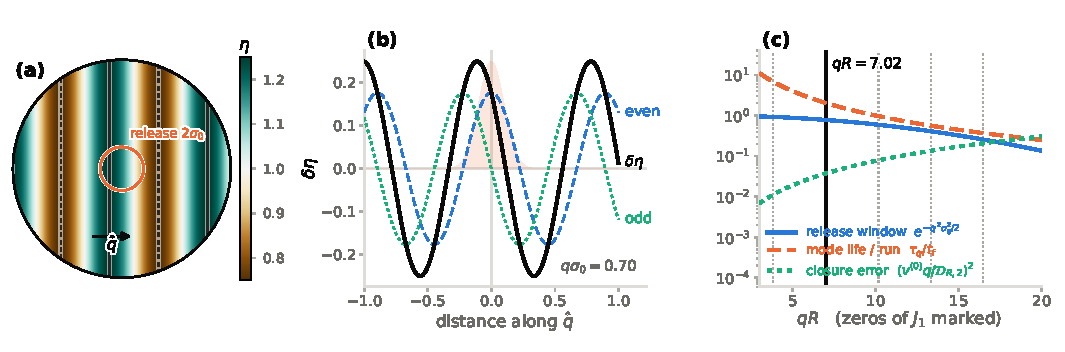
\includegraphics[width=\columnwidth]{figures/figure-2-nutrient-landscape.pdf}
  \caption{Why this mode.  (a) The landscape on the arena and (b) its cut
  along $\hat q$, both reproduced from Fig.~\ref{fig:case1-validation} for
  reference.  (c) Admissible modes are the zeros of $J_1$ (dotted), where the
  disk average of $\delta\eta$ vanishes.  Climbing that ladder, the release
  window falls, the closure error rises and the mode lifetime shrinks toward
  the run time; the second zero (solid line) is the only rung where all three
  are comfortable.}
  \label{fig:landscape}
\end{figure}

\subsection{Calibrating the sensitivities}


The nine sensitivities are calibrated rather than inherited from any organism,
since what this paper compares is rules.  The choice is still constrained.
Each response is linear in its own coefficient, so the only freedom is where
to place a case along its ray $(u_\rho,u_p)$ of density and polarity response
per unit sensitivity, and the ratio $u_\rho/u_p$ is fixed by the physics.  It
spans a factor $19$ across the nine, so matching the density panels exactly
would spread the polarity panels by $19$, and the reverse.  Setting each
sensitivity to $g/\sqrt{u_\rho u_p}$ splits the difference, leaving both
fields spread by only $\sqrt{19}=4.3$---close enough for one linear colour
scale to carry both.  Cases 4 and 8 are then held at
$\lambda^{(\cdot)}=D_R^{(\cdot)}/(1-\Pturn)$ and Case 9 at
$\chi=D_R^{(\zp)}$, which turns the exact degeneracies $2\!\equiv\!4$ and
$6\!\equiv\!8$ into numerical checks.

Visibility costs linearity.  Cases 2 and 4 need the largest fractional
modulation of the coefficient they act on, $D_R^{(\eta)}\varepsilon/D_R^{(0)}=0.24$,
against $0.12$ for Case 5 and below $0.09$ for the rest, so their own
$\ord(\varepsilon^{2})$ error is the largest of the nine.  The quantitative
agreement quoted below therefore rests on the strong rules; the weak ones are
read as shapes.

\subsection{Scope}


Two further checks address the analytic structure rather than any single case.
Integrating the closed system directly in a linear landscape, with no
adiabatic elimination anywhere, recovers $D_{\mathrm{eff}}^{(0)}$ and the
centroid velocity of Eq.~\eqref{eq:pulse-drift} for all nine rules---Cases 1
and 5 giving an identically vanishing drift, as predicted.  The divergence
$\mathcal K$ between two strategies is quadratic where the fields are linear,
so every transient exponent doubles and a detection needs
$M\gtrsim\mathcal K^{-1}$ tracked cells; measured exponents are
$1.95$--$1.97$, $3.91$--$3.96$ and $5.94$ against the predicted $2$, $4$
and $6$.  At fixed cost $Mt$ the evidence grows as $t^{2n-1}$, so watching
longer always beats tracking more.

The scope of all this is three parameter sets and three landscapes, each
inside its own wall-free window, which must be rechecked for any other.

\section{Remaining response mechanisms}
\label{app:remaining-cases}

\begin{figure*}[tp]
 \centering
 \includegraphics[height=0.88\textheight]{../simulation/results/figures/supplementary/figure-s01-cases-2-9-summary.pdf}
 \caption{Three descriptions reproduce the eight remaining response
 mechanisms, all at $t=5\times10^{-3}$.  Columns are particles, the polar PDE
 and the Fourier solution, for density (left) and polarity (right).  Each
 observable has one shared linear scale, so what differs between rows is the
 shape of the response, not its size.  Lines mark nutrient crests and troughs
 as in Fig.~\ref{fig:landscape}.}
 \label{fig:remaining-cases}
\end{figure*}


Figure~\ref{fig:remaining-cases} compares Cases 2--9 using the parameters and
initial condition of Fig.~\ref{fig:case1-validation}.  Each row is one
mechanism; the columns are particles, the polar PDE and the Fourier solution;
every panel is at the common time $t=5\times10^{-3}$ ($t\DR=1.78$).  One
linear scale is shared by all density panels and another by all polarity
panels, with the same limits and spatial window as
Fig.~\ref{fig:case1-validation} and both supplementary videos.

Reading the rows against that common scale is the point of the figure.  With
the sensitivities calibrated as in Sec.~\ref{sec:model-comparison}, no
mechanism is off-scale and none is invisible, so what differs between rows is
the \emph{shape} of the response, not its size.  Cases 2 and 4 remain
indistinguishable, as do Cases 6, 8 and 9 in density---the model's own
degeneracies, reproduced by all three solvers.  Supplementary Video~2 shows
the full evolution.


\begin{thebibliography}{4}

\bibitem{berg1972}
H.~C. Berg and D.~A. Brown,
``Chemotaxis in \textit{Escherichia coli} analysed by three-dimensional
tracking,'' Nature \textbf{239}, 500--504 (1972).

\bibitem{schnitzer1993}
M.~J. Schnitzer,
``Theory of continuum random walks and application to chemotaxis,''
Phys. Rev. E \textbf{48}, 2553--2568 (1993).

\bibitem{tailleur2008}
J. Tailleur and M.~E. Cates,
``Statistical mechanics of interacting run-and-tumble bacteria,''
Phys. Rev. Lett. \textbf{100}, 218103 (2008).

\bibitem{betancourt2026}
J.~M. Betancourt, M.~P. Leighton, T.~Emonet, B.~B. Machta, and M.~C. Abbott,
``Discrete turn strategies emerge in information-limited navigation,''
arXiv:2602.23324v2 (2026).

\bibitem{wilson2011}
L.~G. Wilson, V.~A. Martinez, J.~Schwarz-Linek, J.~Tailleur, G.~Bryant,
P.~N. Pusey, and W.~C.~K. Poon,
``Differential dynamic microscopy of bacterial motility,''
Phys. Rev. Lett. \textbf{106}, 018101 (2011).

\bibitem{martinez2012}
V.~A. Martinez, R.~Besseling, O.~A. Croze, J.~Tailleur, M.~Reufer,
J.~Schwarz-Linek, L.~G. Wilson, M.~A. Bees, and W.~C.~K. Poon,
``Differential dynamic microscopy: a high-throughput method for characterizing
the motility of microorganisms,''
Biophys. J. \textbf{103}, 1637 (2012).

\bibitem{waite2018}
A.~J. Waite, N.~W. Frankel, and T.~Emonet,
``Behavioral variability and phenotypic diversity in bacterial chemotaxis,''
Annu. Rev. Biophys. \textbf{47}, 595 (2018).

\bibitem{ni2020}
B.~Ni, R.~Colin, H.~Link, R.~G. Endres, and V.~Sourjik,
``Growth-rate dependent resource investment in bacterial motile behavior
quantitatively follows potential benefit of chemotaxis,''
Proc. Natl. Acad. Sci. U.S.A. \textbf{117}, 595 (2020).

\end{thebibliography}

\end{document}
